\chapter{Specifica dei casi d'uso}

\section{Introduzione}
In questo documento sono analizzati ed elencati gli attori ed i casi d'uso del sistema.
Scopo del documento è la dettagliata descrizione delle modalità di interazione tra le diverse entità presenti ed il sistema.
Ciò permetterà di mettere in evidenza eventuali conflitti tra i requisiti del sistema stesso.
Tale analisi e descrizione dei casi d'uso verrà presentata tramite grafici che seguono lo standard UML.

\noindent
Si utilizzeranno le seguenti convenzioni:
\begin{itemize}
	\item Nei casi in cui più attori possono accedere ad un determinato caso d’uso, ma quest'ultimo è rivolto principalmente ad un solo attore, non verranno elencati tutti gli altri.

	\item Non verranno riportati tutti gli attori che hanno accesso ad un determinato caso d'uso, ma solo l'attore più generico.
	
	\item Nei diagrammi dei casi d'uso non viene riportato l'identificatore del singolo caso d'uso ma solo il titolo, per facilitarne la lettura.

	\item Nella descrizione dei flussi dei casi d'uso, si assume che sia sempre possibile tornare al passo precedente che richiede interazione con la persona, ad eccezione dei passi in cui si è data una conferma.

	\item Nella descrizione dei flussi alternativi dei casi d'uso, quando si indica la modifica di alcuni punti e non si nominano gli altri, si assume che gli altri rimangano immutati.
\end{itemize}

\section{Elenco degli attori}
Gli attori che interagiscono con il portale sono elencati di seguito:
\begin{itemize}
	\item \newListItem{att:visitatore}{\formattaAtt}{Visitatore}
	\item \newListItem{att:figuraPubblicaAutenticata}{\formattaAtt}{Figura Pubblica Autenticata}
	\item \newListItem{att:figuraAmministrativa}{\formattaAtt}{Figura Amministrativa}
	\item \newListItem{att:utente}{\formattaAtt}{Utente}
	\item \newListItem{att:produttore}{\formattaAtt}{Produttore}
	\item \newListItem{att:redattore}{\formattaAtt}{Redattore}
	\item \newListItem{att:assistente}{\formattaAtt}{Assistente}
	\item \newListItem{att:moderatore}{\formattaAtt}{Moderatore}
	\item \newListItem{att:amministratore}{\formattaAtt}{Amministratore}
	\item \newListItem{att:cms}{\formattaAtt}{CMS}
\end{itemize}
La gerarchia degli attori è mostrata nel seguente diagramma UML:
\begin{center}
   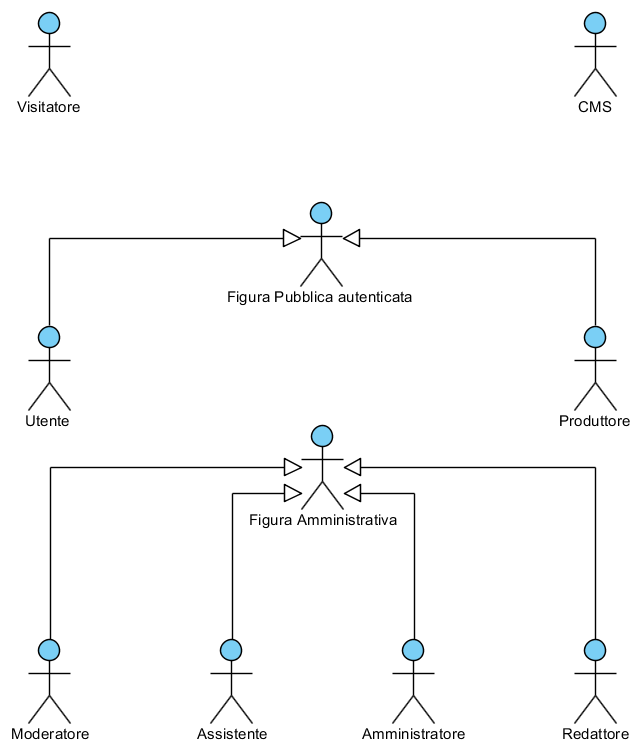
\includegraphics[width=\textwidth]{assets/visualParadigm/cu/SchemaAttori}
\end{center}

\section{Specifica degli attori}
Gli attori che interagiscono con il portale sono descritti di seguito:
\attTab{att:visitatore}{-}{\glsdesc*{visitatore}}

\vspaceTab

\attTab{att:figuraPubblicaAutenticata}{-}{\glsdesc*{figuraPubblicaAutenticata}}

\vspaceTab

\attTab{att:figuraAmministrativa}{-}{\glsdesc*{figuraAmministrativa}}

\vspaceTab

\attTab{att:utente}{\getTitletodesc{att:figuraPubblicaAutenticata}}{\glsdesc*{utente}}

\vspaceTab

\attTab{att:produttore}{\getTitletodesc{att:figuraPubblicaAutenticata}}{\glsdesc*{produttore}}

\vspaceTab

\attTab{att:redattore}{\getTitletodesc{att:figuraAmministrativa}}{\glsdesc*{redattore}}

\vspaceTab

\attTab{att:assistente}{\getTitletodesc{att:figuraAmministrativa}}{\glsdesc*{assistente}}

\vspaceTab

\attTab{att:moderatore}{\getTitletodesc{att:figuraAmministrativa}}{\glsdesc*{moderatore}}

\vspaceTab

\attTab{att:amministratore}{\getTitletodesc{att:figuraAmministrativa}}{\glsdesc*{amministratore}}

\vspaceTab

\attTab{att:cms}{-}{\glsdesc*{cmsdef}}

\section{Identificativo dei casi d'uso} %(vengono usati per definire l'ID, non ha senso metterli dopo la struttura ID)
Di seguito è spiegato come interpretare l'identificativo dei casi d'uso:
\begin{center}
	\use{categoria}{caso}%{[sottoreq]}{[\dots]}
\end{center}

\noindent
Segue una descrizione di ogni campo utilizzato nell'identificatore:
\begin{itemize}
	\item La \campiIdReq{categoria} è una lettera utilizzata per raggruppare i casi d'uso con scopi simili.
	Le categorie sono le seguenti:
	\begin{enumerateIndLabel}{\textsf{\Alph*}}{\Alph*}
		\item Autenticazione. \label{pkg:autenticazione}
		\item Gestione iscrizioni. \label{pkg:iscrizione}
		\item Gestione vetrina. \label{pkg:vetrina} 
		\item Gestione notizie. \label{pkg:notizie}
		\item Gestione suggerimenti. \label{pkg:suggerimenti}
		\item Gestione account. \label{pkg:account}
		\item Gestione valutazioni. \label{pkg:gestionevalutazione}
		\item Gestione recensioni. \label{pkg:gestionerecensione}
		\item Interazione tra figure. \label{pkg:interazione}
		\item Gestione ticket. \label{pkg:gestioneticket}
		\item Ricerca contenuti. \label{pkg:ricerca}
		\item Gestione prodotti mancanti. \label{pkg:prodottimancanti}
		\item Visualizzazione contenuti pubblici. \label{pkg:visualizzazione}
	\end{enumerateIndLabel}

	\item Il campo \campiIdReq{caso} è un numero progressivo utilizzato per identificare in modo univoco un caso d'uso all'interno della sua categoria.
\end{itemize}

\section{Elenco dei casi d'uso}
Vengono di seguito elencati i casi d'uso:
\begin{itemize} 
	\setCatCU{\ref*{pkg:autenticazione}}%A
	\item \newListItem{cu:login}{\formattaCU}{Login}
	\item \newListItem{cu:loginAmm}{\formattaCU}{Login Figure Amministrative}
	\item \newListItem{cu:logout}{\formattaCU}{Logout}

	\setCatCU{\ref*{pkg:iscrizione}}%B
	\item \newListItem{cu:iscrizionePortale}{\formattaCU}{Iscrizione tramite modulo}
	\item \newListItem{cu:iscrizioneSocial}{\formattaCU}{Iscrizione tramite Social Network}
	\item \newListItem{cu:iscrizioneApprovazione}{\formattaCU}{Iscrizione tramite approvazione}
	\item \newListItem{cu:approvazioneIscrizione}{\formattaCU}{Approvazione iscrizione}

	\setCatCU{\ref*{pkg:vetrina}}%C
	\item \newListItem{cu:personalizzaVetrinaInsDesc}{\formattaCU}{Inserimento descrizione}
	\item \newListItem{cu:personalizzaVetrinaModDesc}{\formattaCU}{Modifica descrizione}
	\item \newListItem{cu:personalizzaVetrinaInsImg}{\formattaCU}{Inserimento immagine}
	\item \newListItem{cu:personalizzaVetrinaDelImg}{\formattaCU}{Rimozione immagine}
	\item \newListItem{cu:personalizzaVetrinaInsProd}{\formattaCU}{Inserimento scheda prodotto}
	\item \newListItem{cu:personalizzaVetrinaModProd}{\formattaCU}{Modifica scheda prodotto}
	\item \newListItem{cu:statistichePrivateVetrina}{\formattaCU}{Mostra statistiche private della vetrina}


	\setCatCU{\ref*{pkg:notizie}}%D
	\item \newListItem{cu:inserimentoNotizia}{\formattaCU}{Inserimento notizia}
	\item \newListItem{cu:modificaNotizia}{\formattaCU}{Modifica notizia}
	\item \newListItem{cu:rimozioneNotizia}{\formattaCU}{Rimozione notizia}

	\setCatCU{\ref*{pkg:suggerimenti}}%E
	\item \newListItem{cu:suggerimentoProdotti}{\formattaCU}{Suggerimento prodotti}
	\item \newListItem{cu:notizieSimili}{\formattaCU}{Suggerimento notizie}
	
	\setCatCU{\ref*{pkg:account}}%F
	\item \newListItem{cu:modificaProfilo}{\formattaCU}{Modifica del proprio profilo}
	\item \newListItem{cu:inserisciImgProfilo}{\formattaCU}{Inserimento immagine profilo proprio}
	\item \newListItem{cu:rimuoviImgProfilo}{\formattaCU}{Rimozione immagine profilo proprio}
	\item \newListItem{cu:modificaImpostazioni}{\formattaCU}{Modifica delle proprie impostazioni}
	\item \newListItem{cu:rimozioneAccountProprio}{\formattaCU}{Rimozione account proprio}
	\item \newListItem{cu:rimozioneAccountAltrui}{\formattaCU}{Rimozione account altrui}
	\item \newListItem{cu:modificaPrivilegiAccount}{\formattaCU}{Modifica privilegi di un account}


	\setCatCU{\ref*{pkg:gestionevalutazione}}%G
	\item \newListItem{cu:inserisciValutazioneProdotto}{\formattaCU}{Inserimento valutazione}
	\item \newListItem{cu:modificaValutazioneProdotto}{\formattaCU}{Modifica valutazione}

	\setCatCU{\ref*{pkg:gestionerecensione}}%H
	\item \newListItem{cu:inserisciRecensioneProdotto}{\formattaCU}{Inserimento recensione}
	\item \newListItem{cu:modificaRecensioneProdotto}{\formattaCU}{Modifica recensione propria}
	\item \newListItem{cu:eliminaRecensioneProdotto}{\formattaCU}{Rimozione recensione propria}
	\item \newListItem{cu:commentoRecensione}{\formattaCU}{Commento a recensione}
	\item \newListItem{cu:giudizioRecensione}{\formattaCU}{Giudizio recensione}
	\item \newListItem{cu:modificaGiudizioRecensione}{\formattaCU}{Modifica giudizio recensione}
	\item \newListItem{cu:segnalazioneContenutiInap}{\formattaCU}{Segnalazione contenuti inappropriati}
	\item \newListItem{cu:mostraSegnContenutiInap}{\formattaCU}{Mostra segnalazioni contenuti}
	\item \newListItem{cu:rimozioneContenutiInap}{\formattaCU}{Rimozione contenuti inappropriati}

	\setCatCU{\ref*{pkg:interazione}}%I
	\item \newListItem{cu:followAccount}{\formattaCU}{Follow account}
	\item \newListItem{cu:unFollowAccount}{\formattaCU}{Unfollow account}

	\setCatCU{\ref*{pkg:gestioneticket}}%J
	\item \newListItem{cu:ticketInvio}{\formattaCU}{Invio di un ticket}
	\item \newListItem{cu:ticketRisposta}{\formattaCU}{Risposta ad un ticket}
	\item \newListItem{cu:ticketChiudi}{\formattaCU}{Chiusura di un ticket}
	\item \newListItem{cu:ticketLettura}{\formattaCU}{Lettura di un ticket}

	\setCatCU{\ref*{pkg:ricerca}}%K
	\item \newListItem{cu:ricercaProdotto}{\formattaCU}{Ricerca prodotto}
	\item \newListItem{cu:ricercaProfilo}{\formattaCU}{Ricerca profilo}
	\item \newListItem{cu:ricercaNotizia}{\formattaCU}{Ricerca notizia}

	\setCatCU{\ref*{pkg:prodottimancanti}}%L
	\item \newListItem{cu:richiestaInsProdotto}{\formattaCU}{Richiesta inserimento scheda prodotto}
	\item \newListItem{cu:mostraRichiestaInsProdotto}{\formattaCU}{Mostra richiesta scheda prodotto}
	\item \newListItem{cu:richiestaInsProduttore}{\formattaCU}{Richiesta inserimento produttore e scheda prodotto}

	\setCatCU{\ref*{pkg:visualizzazione}}%M
	\item \newListItem{cu:mostraVetrina}{\formattaCU}{Mostra vetrina}
	\item \newListItem{cu:mostraProdotto}{\formattaCU}{Mostra scheda prodotto}
	\item \newListItem{cu:mostraRecensioniProdotto}{\formattaCU}{Mostra recensioni associate al prodotto}
	\item \newListItem{cu:mostraRecensione}{\formattaCU}{Mostra recensione}
	\item \newListItem{cu:mostraProfilo}{\formattaCU}{Mostra profilo pubblico}
	\item \newListItem{cu:mostraNotizia}{\formattaCU}{Mostra notizia}
	\item \newListItem{cu:mostraAggF}{\formattaCU}{Mostra aggiornamenti dai followed}
\end{itemize}	

%{id}{attori}{pre}{post}{flusso}
\section{Specifica dei casi d'uso}
Vengono di seguito elencate le tabelle che descrivono i casi d'uso, suddivisi per categoria:

\subsection{Autenticazione}
\begin{center}
   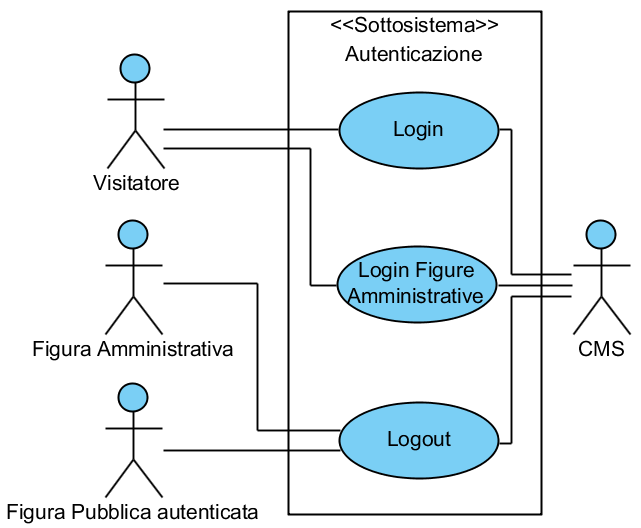
\includegraphics[width=\textwidth]{assets/visualParadigm/cu/Autenticazione}
\end{center}
%*************** LOGIN *****************
\cuTab{cu:login}%
{\getTitletodesc{att:visitatore}}%
{La persona connessa al sito è inizialmente riconosciuta come Visitatore}%
{La persona connessa al sito è ora riconosciuta come Figura Pubblica Autenticata}%
{\begin{enumCU}
	\item Il caso d'uso ha inizio quando un Visitatore richiede di effettuare il login 
	\item Il sistema richiede le credenziali di autenticazione
	\item Il Visitatore inserisce le credenziali di accesso negli appositi campi \label{culogin:3}
	\item Il Visitatore conferma i dati inseriti
	\item Il sistema verifica che i dati inseriti corrispondano ad un account pubblico esistente\label{culogin:5}
	\item Il sistema accetta le credenziali ricevute
\end{enumCU}}%
%
\cuAlternativo{cu:login}
{Flusso alternativo 1}%
{Errore Login}%
{La persona connessa al sito è inizialmente riconosciuta come Visitatore}%
{\postNulle}%
{\begin{enumCU}
	\item Dopo il punto \ref{culogin:5} il sistema rifiuta le credenziali
\end{enumCU}}%
%
\cuAlternativo{cu:login}
{Flusso alternativo 2}%
{Annulla Login}%
{La persona connessa al sito è inizialmente riconosciuta come Visitatore}%
{\postNulle}%
{\begin{enumCU}
		\item Dopo il punto \ref{culogin:3} il Visitatore annulla l'operazione di login
\end{enumCU}}%

\vspaceTab

\cuTab{cu:loginAmm}%
{\getTitletodesc{att:visitatore}}%
{La persona connessa al sito è inizialmente riconosciuta come Visitatore}%
{La persona connessa al sito è ora riconosciuta come Figura Amministrativa}%
{\begin{enumCU}
	\item Il caso d'uso ha inizio quando un Visitatore richiede di effettuare il login 
	\item Il sistema richiede le credenziali di autenticazione
	\item Il Visitatore inserisce le credenziali di accesso negli appositi campi \label{culoginamm:3}
	\item Il Visitatore conferma i dati inseriti
	\item Il sistema verifica che i dati inseriti corrispondano ad un account amministrativo esistente\label{culoginamm:5}
	\item Il sistema accetta le credenziali ricevute
	\item Il sistema invia un codice casuale sul cellulare del Visitatore
	\item Il Visitatore inserisce il codice ricevuto sul cellulare in un apposito campo \label{culoginamm:8}
	\item Il Visitatore conferma il codice inserito
	\item Il sistema verifica che il codice inserito corrisponda a quello inviato \label{culoginamm:10}
	\item Il sistema accetta il codice ricevuto
\end{enumCU}}%
%
\cuAlternativo{cu:loginAmm}
{Flusso alternativo 1}%
{Errore Credenziali}%
{La persona connessa al sito è inizialmente riconosciuta come Visitatore}%
{\postNulle}%
{\begin{enumCU}
	\item Dopo il punto \ref{culoginamm:5} il sistema rifiuta le credenziali
\end{enumCU}}%
%
\cuAlternativo{cu:loginAmm}
{Flusso alternativo 2}%
{Annulla Credenziali}%
{La persona connessa al sito è inizialmente riconosciuta come Visitatore}%
{\postNulle}%
{\begin{enumCU}
		\item Dopo il punto \ref{culoginamm:3} il Visitatore annulla l'operazione di login
\end{enumCU}}%
%
\cuAlternativo{cu:loginAmm}
{Flusso alternativo 3}%
{Errore Codice}%
{La persona connessa al sito è inizialmente riconosciuta come Visitatore}%
{\postNulle}%
{\begin{enumCU}
		\item Dopo il punto \ref{culoginamm:10}, il sistema rifiuta il codice
\end{enumCU}}%
%
\cuAlternativo{cu:loginAmm}
{Flusso alternativo 4}%
{Annulla Codice}%
{La persona connessa al sito è inizialmente riconosciuta come Visitatore}%
{\postNulle}%
{\begin{enumCU}
		\item Dopo il punto \ref{culoginamm:8}, il Visitatore annulla l'operazione di login
\end{enumCU}}%

\vspaceTab

%*************** LOGOUT *****************
\cuTab{cu:logout}
{\getTitletodesc{att:figuraAmministrativa}, \getTitletodesc{att:figuraPubblicaAutenticata}}
{La persona connessa al sito è autenticata}
{La persona connessa al sito non è più autenticata ed è ora un Visitatore}
{\begin{enumCU}
	\item Il caso d'uso ha inizio quando una persona autenticata richiede di effettuare il logout
	\item Il sistema effettua il logout richiesto
\end{enumCU}}

\subsection{Gestione iscrizioni}
\begin{center}
   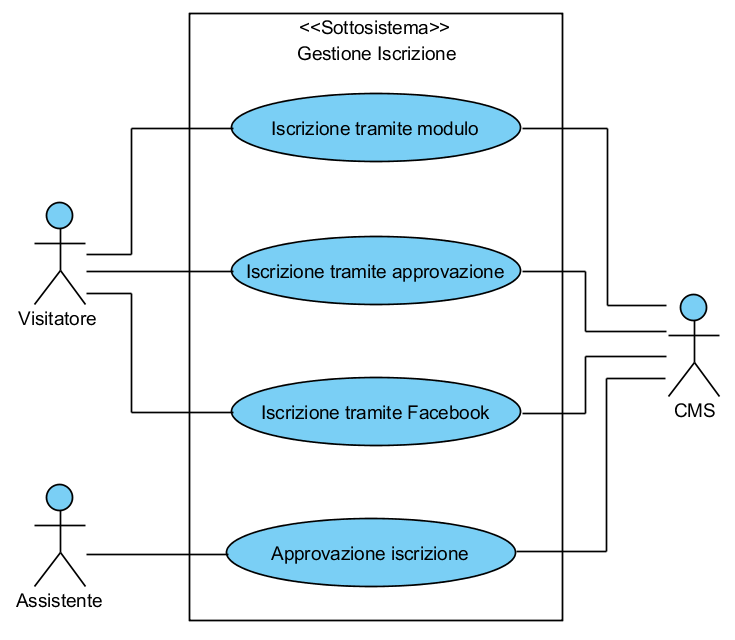
\includegraphics[width=\textwidth]{assets/visualParadigm/cu/GestioneIscrizione}
\end{center}
%*************** ISCRIZIONE PORTALE *****************
\cuTab{cu:iscrizionePortale}
{\getTitletodesc{att:visitatore}}
{La persona connessa al sito è inizialmente riconosciuta come Visitatore}
{La persona ha ora un account proprio, creato con i dati da essa inseriti}
{\begin{enumCU}
	\item Il caso d'uso ha inizio quando un Visitatore richiede di effettuare l'iscrizione
	\item Il sistema richiede i dati richiesti per effettuare l'iscrizione tra cui un identificatore all'interno del sistema
	\item Il Visitatore inserisce i dati richiesti negli appositi campi \label{cuiscr:3}
	\item Il Visitatore conferma i dati inseriti
	\item Il sistema verifica che i dati inseriti siano corretti e che l'identificatore dell'account che si sta creando non sia già presente \label{cuiscr:5}
	\item Il sistema crea un nuovo account con le credenziali ricevute
\end{enumCU}}
%
\cuAlternativo{cu:iscrizionePortale}
{Flusso alternativo 1}%
{Annulla iscrizione}%
{La persona connessa al sito è inizialmente riconosciuta come Visitatore}%
{\postNulle}%
{\begin{enumCU}
		\item Dopo il punto \ref{cuiscr:3} l'utente annulla l'operazione di iscrizione
	\end{enumCU}}%
%
\cuAlternativo{cu:iscrizionePortale}
{Flusso alternativo 2}%
{Errore iscrizione}%
{La persona connessa al sito è inizialmente riconosciuta come Visitatore}%
{\postNulle}%
{\begin{enumCU}
		\item Dopo il punto \ref{cuiscr:5} il sistema rileva un errore nei dati inseriti
	\end{enumCU}}%


\vspaceTab

%%%FORSE DA TOGLIERE -------------------------------------------------------------------------
%Accorpa verificati e non verificati
\cuTab{cu:iscrizioneSocial}
{\getTitletodesc{att:visitatore}}
{La persona è connessa al sito come Visitatore}
{La persona ha ora un account proprio, creato tramite le API messe a disposizione dal Social Network utilizzato durante l'iscrizione}
{\begin{enumCU}
		\item Il caso d'uso ha inizio quando un Visitatore richiede di effettuare l'iscrizione tramite un Social Network
		\item Il sistema richiede le credenziali di accesso del Social Network scelto
		\item Il Visitatore inserisce i dati richiesti \label{cuiscrappsocial:3}
		\item Il Visitatore conferma i dati inseriti \label{cuiscrappsocial:5}
		\item Il Il sistema crea un nuovo account con le credenziali ricevute
	\end{enumCU}}

\vspaceTab
%
\cuAlternativo{cu:iscrizioneSocial}
{Flusso alternativo 1}%
{Annulla iscrizione}%
{La persona connessa al sito è inizialmente riconosciuta come Visitatore}%
{\postNulle}%
{\begin{enumCU}
		\item Dopo il punto \ref{cuiscrappsocial:3} il Visitatore annulla l'operazione di iscrizione
	\end{enumCU}}%
%
\cuAlternativo{cu:iscrizioneSocial}
{Flusso alternativo 2}%
{Errore iscrizione}%
{La persona connessa al sito è inizialmente riconosciuta come Visitatore}%
{\postNulle}%
{\begin{enumCU}
		\item Dopo il punto \ref{cuiscrappsocial:5} il sistema rileva un errore nei dati inseriti
	\end{enumCU}}%

\vspaceTab

%*************** ISCRIZIONE CON APPROVAZIONE *****************
\cuTab{cu:iscrizioneApprovazione}
{\getTitletodesc{att:visitatore}}
{La persona connessa al sito è inizialmente riconosciuta come Visitatore}
{Viene inserita nel sistema una richiesta di creazione di un account di tipo Produttore con i dati inseriti dalla persona}
{\begin{enumCU}
	\item Il caso d'uso ha inizio quando un Visitatore richiede di effettuare l'iscrizione tramite approvazione
	\item Il sistema richiede i dati richiesti per effettuare l'iscrizione  tra cui un identificatore all'interno del sistema
	\item Il Visitatore inserisce i dati richiesti negli appositi campi \label{cuiscrapp:3}
	\item Il Visitatore conferma i dati inseriti
	\item Il sistema verifica che i dati inseriti siano corretti e che l'identificatore dell'account che si sta creando non sia già presente \label{cuiscrapp:5}
	\item Il sistema crea una richiesta di iscrizione con le credenziali ricevute
\end{enumCU}}
%
\cuAlternativo{cu:iscrizioneApprovazione}
{Flusso alternativo 1}%
{Annulla iscrizione}%
{La persona connessa al sito è inizialmente riconosciuta come Visitatore}%
{\postNulle}%
{\begin{enumCU}
		\item Dopo il punto \ref{cuiscrapp:3} il Visitatore annulla l'operazione di iscrizione
	\end{enumCU}}%
%
\cuAlternativo{cu:iscrizioneApprovazione}
{Flusso alternativo 2}%
{Errore iscrizione}%
{La persona connessa al sito è inizialmente riconosciuta come Visitatore}%
{\postNulle}%
{\begin{enumCU}
		\item Dopo il punto \ref{cuiscrapp:5} il sistema rileva un errore nei dati inseriti
	\end{enumCU}}%

\vspaceTab

%***************  APPROVAZIONE DI UNA RICHIESTA DI ISCRIZIONE *****************
\cuTab{cu:approvazioneIscrizione}
{\getTitletodesc{att:assistente}}
{La persona connessa al sito è autenticata e ha i privilegi di  Assistente. Nel sistema è presente almeno una richiesta di creazione di un account}
{Il Visitatore che ha effettuato la richiesta ha ora un account di tipo Produttore. Nel sistema non è più presente la richiesta}
{\begin{enumCU}
	\item Il caso d'uso ha inizio quando una persona con privilegi di Assistente richiede di controllare una richiesta di iscrizione
	\item Il sistema mostra all'Assistente le richieste presenti nel sistema e chiede di selezionarne una\label{cuappriscr:0}
	\item L'Assistente seleziona una richiesta di iscrizione
	\item Il sistema mostra all'Assistente la richiesta da lui selezionata\label{cuappriscr:1}
	\item L'Assistente approva la richiesta di iscrizione
	\item Il sistema rimuove la richiesta selezionata dall'Assistente
\end{enumCU}}
%
\cuAlternativo{cu:approvazioneIscrizione}
{Flusso alternativo 1}%
{Richiesta rifiutata}%
{La persona connessa al sito è autenticata e ha i privilegi di  Assistente. Nel sistema è presente almeno una richiesta di creazione di un account}%
{Nel sistema non è più presente la richiesta selezionata}%
{\begin{enumCU}
		\item Dopo il punto \ref{cuappriscr:1} l'Assistente rifiuta la richiesta di creazione dell'account
		\item Il sistema rimuove la richiesta selezionata dall'Assistente
\end{enumCU}}%
%
\cuAlternativo{cu:approvazioneIscrizione}
{Flusso alternativo 2}%
{Annulla operazione di selezione}%
{La persona connessa al sito è autenticata e ha i privilegi di  Assistente. Nel sistema è presente almeno una richiesta di creazione di un account}%
{\postNulle}%
{\begin{enumCU}
		\item Dopo il punto \ref{cuappriscr:0} l'Assistente annulla l'operazione di selezione
\end{enumCU}}%

\subsection{Gestione vetrina}
\begin{center}
   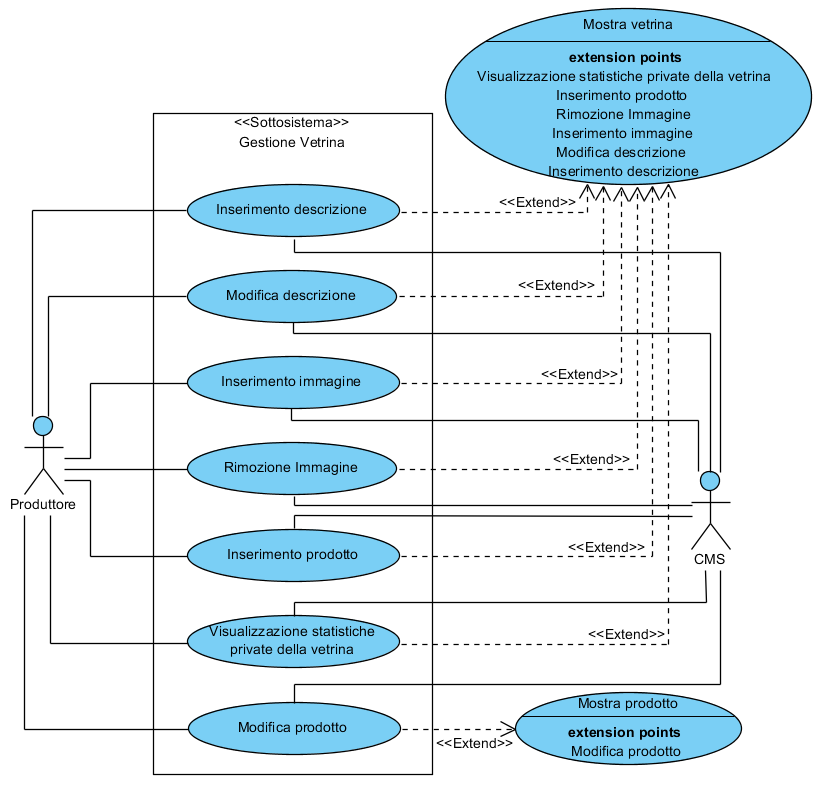
\includegraphics[width=\textwidth]{assets/visualParadigm/cu/GestioneVentrina}
\end{center}
%***************  INSERISCI DESCRIZIONE IN VETRINA *****************
\cuTab{cu:personalizzaVetrinaInsDesc}
{\getTitletodesc{att:produttore}}
{La persona connessa al sito è autenticata e ha i privilegi di Produttore. Nel sistema non è presente la descrizione della vetrina di quel Produttore. Il sistema sta mostrando alla persona la sua vetrina}
{Nel sistema è presente la descrizione della vetrina del Produttore, inserita dalla persona}
{\begin{enumCU}
		\item Il caso d'uso ha inizio quando un Produttore richiede di inserire la descrizione della sua vetrina
		\item Il sistema richiede il testo da inserire come descrizione 
		\item Il Produttore inserisce la descrizione nell'apposito campo\label{cuinsdescr:2}
		\item Il Produttore conferma il testo inserito
		\item Il sistema memorizza il testo inserito
	\end{enumCU}}
%
\cuAlternativo{cu:personalizzaVetrinaInsDesc}
{Flusso alternativo 1}%
{Annulla inserimento}%
{La persona connessa al sito è autenticata e ha i privilegi di Produttore. Nel sistema non è presente la descrizione della vetrina di quel Produttore. Il sistema sta mostrando alla persona la sua vetrina}%
{\postNulle}%
{\begin{enumCU}
		\item Dopo il punto \ref{cuinsdescr:2} il Produttore annulla l'inserimento della descrizione
	\end{enumCU}}%

\vspaceTab

\cuTab{cu:personalizzaVetrinaModDesc}
{\getTitletodesc{att:produttore}}
{La persona connessa al sito è autenticata e ha i privilegi di Produttore. Nel sistema è presente la descrizione della vetrina di quel Produttore. Il sistema sta mostrando alla persona la sua vetrina}
{Nel sistema è presente la descrizione della vetrina del Produttore, inserita dalla persona}
{\begin{enumCU}
		\item Il caso d'uso ha inizio quando un Produttore richiede di modificare la descrizione della sua vetrina
		\item Il sistema richiede il testo da inserire come descrizione, il campo in cui inserire il testo è precompilato con la descrizione già presente nel sistema 
		\item Il Produttore inserisce la descrizione nell'apposito campo\label{cumoddescr:2}
		\item Il Produttore conferma il testo inserito
		\item Il sistema memorizza il testo inserito
	\end{enumCU}}
%
\cuAlternativo{cu:personalizzaVetrinaModDesc}
{Flusso alternativo 1}%
{Annulla modifica}%
{La persona connessa al sito è autenticata e ha i privilegi di Produttore. Nel sistema è presente la descrizione della vetrina di quel Produttore. Il sistema sta mostrando alla persona la sua vetrina}%
{\postNulle}%
{\begin{enumCU}
		\item Dopo il punto \ref{cumoddescr:2} il Produttore annulla la modifica della descrizione
	\end{enumCU}}%

\vspaceTab

%***************  INSERISCI IMMAGINE IN VETRINA *****************
\cuTab{cu:personalizzaVetrinaInsImg}
{\getTitletodesc{att:produttore}}
{La persona connessa al sito è autenticata e ha i privilegi di Produttore. Il sistema sta mostrando alla persona la sua vetrina}
{Nel sistema è presente l'immagine della vetrina del Produttore, inserita dalla persona}
{\begin{enumCU}
		\item Il caso d'uso ha inizio quando un Produttore richiede di inserire l'immagine della sua vetrina
		\item Il sistema richiede il percorso nel file system, o nella rete, dell'immagine da inserire 
		\item Il Produttore inserisce il percorso dell'immagine nell'apposito campo\label{cuinsimm:2}
		\item Il Produttore conferma il percorso dell'immagine inserito\label{cuinsimm:3}
		\item Il sistema scarica e memorizza l'immagine impostandola come immagine della vetrina del Produttore
	\end{enumCU}}
%
\cuAlternativo{cu:personalizzaVetrinaInsImg}
{Flusso alternativo 1}%
{Errore inserimento}%
{La persona connessa al sito è autenticata e ha i privilegi di Produttore. Il sistema sta mostrando alla persona la sua vetrina}%
{\postNulle}%
{\begin{enumCU}
		\item Dopo il punto \ref{cuinsimm:3} il sistema non riesce a trovare, scaricare o inserire correttamente l'immagine
	\end{enumCU}}%
%
\cuAlternativo{cu:personalizzaVetrinaInsImg}
{Flusso alternativo 2}%
{Annulla inserimento}%
{La persona connessa al sito è autenticata e ha i privilegi di Produttore. Il sistema sta mostrando alla persona la sua vetrina}%
{\postNulle}%
{\begin{enumCU}
		\item Dopo il punto \ref{cuinsimm:2} il produttore annulla l'inserimento dell'immagine
	\end{enumCU}}%

\vspaceTab

\cuTab{cu:personalizzaVetrinaDelImg}
{\getTitletodesc{att:produttore}}
{La persona connessa al sito è autenticata e ha i privilegi di Produttore. Nel sistema è presente l'immagine della vetrina del Produttore. Il sistema sta mostrando alla persona la sua vetrina}
{Nel sistema non è presente l'immagine della vetrina del Produttore}
{\begin{enumCU}
		\item Il caso d'uso ha inizio quando un Produttore richiede di rimuovere l'immagine della sua vetrina
		\item Il sistema richiede di confermare l'operazione \label{cudelimm:2}
		\item Il Produttore conferma l'operazione
		\item Il sistema rimuove l'immagine della vetrina del produttore
	\end{enumCU}}

\vspaceTab

%***************  INSERISCI PRODOTTO IN VETRINA *****************
\cuTab{cu:personalizzaVetrinaInsProd}
{\getTitletodesc{att:produttore}}
{La persona connessa al sito è autenticata e ha i privilegi di Produttore. Il sistema sta mostrando alla persona la sua vetrina}
{Nella vetrina del Produttore è presente la scheda del prodotto inserito}
{\begin{enumCU}
		\item Il caso d'uso ha inizio quando un Produttore richiede di inserire un prodotto nella sua vetrina
		\item Il sistema richiede di compilare la scheda del prodotto da inserire
		\item Il Produttore inserisce i dati richiesti\label{cuinsimmpro:1}
		\item Il Produttore conferma i dati inseriti 
		\item Il sistema richiede almeno un percorso nel file system, o nella rete, dell'immagine del prodotto da inserire
		\item Il Produttore inserisce nell'apposito campo uno o più percorsi  delle immagini che vuole inserire\label{cuinsimmpro:2}
		\item Il Produttore conferma i percorsi inseriti\label{cuinsimmpro:3}
		\item Il sistema memorizza i dati e i percorsi inseriti e scarica le immagini nel sistema
	\end{enumCU}}
%
\cuAlternativo{cu:personalizzaVetrinaInsProd}
{Flusso alternativo 1}%
{Errore inserimento}%
{La persona connessa al sito è autenticata e ha i privilegi di Produttore. Il sistema sta mostrando alla persona la sua vetrina}%
{\postNulle}%
{\begin{enumCU}
		\item Dopo il punto \ref{cuinsimmpro:3} il sistema non riesce a trovare, scaricare o inserire correttamente una o più immagini
	\end{enumCU}}%
%
\cuAlternativo{cu:personalizzaVetrinaInsProd}
{Flusso alternativo 2}%
{Annulla inserimento}%
{La persona connessa al sito è autenticata e ha i privilegi di Produttore. Il sistema sta mostrando alla persona la sua vetrina}%
{\postNulle}%
{\begin{enumCU}
		\item Dopo il punto \ref{cuinsimmpro:2} o dopo il punto \ref{cuinsimmpro:1} il Produttore annulla l'inserimento della scheda prodotto
	\end{enumCU}}%

\vspaceTab

%***************  MODIFICA PRODOTTO IN VETRINA *****************
\cuTab{cu:personalizzaVetrinaModProd}
{\getTitletodesc{att:produttore}}
{La persona connessa al sito è autenticata e ha i privilegi di Produttore. Il sistema sta mostrando alla persona la scheda di un prodotto presente nella sua vetrina}%
{Nella vetrina del Produttore è stata modificara la scheda del prodotto selezionato}
{\begin{enumCU}
		\item Il caso d'uso ha inizio quando un Produttore richiede di modificare la scheda del prodotto che sta visualizzando
		\item Il sistema richiede di compilare la scheda prodotto, precompilata con i dati già presenti nel sistema
		\item Il Produttore inserisce i dati richiesti\label{cumodprodelim:1}
		\item Il Produttore conferma i dati inseriti
		\item Il sistema mostra le immagini del prodotto presenti, con la possibilità di eliminarle, e mostra i campi per aggiungere i percorsi nel file system, o nella rete, di altre immagini da aggiungere\label{cumodprodelim:3}
		\item Il Produttore inserisce i percorsi nel file system delle immagini che intende aggiungere
		\item Il Produttore conferma i percorsi inseriti\label{cumodprodelim:2}
		\item Il sistema memorizza i dati e i percorsi inseriti e scarica le immagini nel sistema
	\end{enumCU}} %%SETTARE UN PRODOTTO COME FUORI PRODUZIONE&&
%
\cuAlternativo{cu:personalizzaVetrinaModProd}
{Flusso alternativo 1}%
{Elimina immagine}%
{La persona connessa al sito è autenticata e ha i privilegi di Produttore. Il sistema sta mostrando alla persona la scheda di un prodotto con almeno due immagini presente nella sua vetrina}
{Nel sistema non è più presente l'immagine selezionata}%
{\begin{enumCU}
		\item Dopo il punto \ref{cumodprodelim:3} il Produttore seleziona un'immagine
		\item Il Produttore richiede la rimozione dell'immagine
		\item Il sistema accetta l'operazione
	\end{enumCU}}%
%
\cuAlternativo{cu:personalizzaVetrinaModProd}
{Flusso alternativo 2}%
{Annulla Modifica}%
{La persona connessa al sito è autenticata e ha i privilegi di Produttore. Il sistema sta mostrando alla persona la scheda di un prodotto presente nella sua vetrina}%
{\postNulle}%
{\begin{enumCU}
		\item Dopo il punto \ref{cumodprodelim:2} o dopo il punto \ref{cumodprodelim:1} il Produttore annulla l'inserimento della scheda del prodotto
	\end{enumCU}}%

\vspaceTab

%***************  STATISTICHE PRIVATE VETRINA *****************
\cuTab{cu:statistichePrivateVetrina}
{\getTitletodesc{att:produttore}}
{La persona connessa al sito è autenticata e ha i privilegi di Produttore. Il sistema sta mostrando alla persona la sua vetrina}
{Il sistema sta mostrando al Produttore le statistiche private della propria vetrina}
{\begin{enumCU}
		\item Il caso d'uso ha inizio quando un Produttore richiede di accedere alle statistiche private della sua vetrina
		\item Il sistema mostra al Produttore le statistiche della sua vetrina
	\end{enumCU}}

\subsection{Gestione notizie}
\begin{center}
   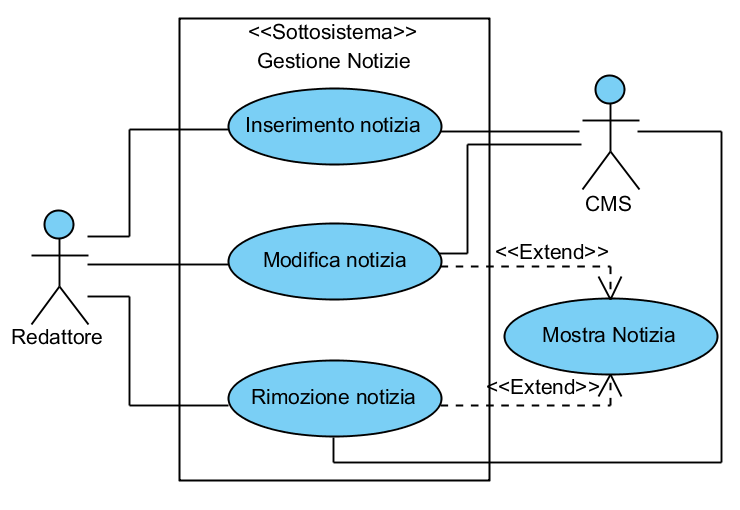
\includegraphics[width=\textwidth]{assets/visualParadigm/cu/GestioneNotizie}
\end{center}
%
%***************  INSERIMENTO NOTIZIA *****************
\cuTab{cu:inserimentoNotizia}
{\getTitletodesc{att:redattore}}
{La persona connessa al sito è autenticata e ha i privilegi di Redattore}
{Nel sistema è presente la notizia inserita}
{\begin{enumCU}
	\item Il caso d'uso ha inizio quando un Redattore richiede di inserire una notizia  
	\item Il sistema richiede di compilare i campi necessari all'inserimento della notizia
	\item Il Redattore inserisce i dati richiesti \label{cuinsnot:2}
	\item Il Redattore conferma i dati richiesti
	\item Il sistema memorizza i dati inseriti e crea una nuova notizia
\end{enumCU}}
%
\cuAlternativo{cu:inserimentoNotizia}
{Flusso alternativo 1}%
{Annulla inserimento}%
{La persona connessa al sito è autenticata e ha i privilegi di Redattore}%
{\postNulle}%
{\begin{enumCU}
		\item Dopo il punto \ref{cuinsnot:2} il Redattore annulla l'inserimento della notizia
	\end{enumCU}}%

\vspaceTab

%***************  MODIFICA NOTIZIA *****************
\cuTab{cu:modificaNotizia}
{\getTitletodesc{att:redattore}}
{La persona connessa al sito è autenticata e ha i privilegi di Redattore. Il sistema sta mostrando alla persona una notizia}
{Nel sistema la notizia viene modificata correttamente}
{\begin{enumCU}
	\item Il caso d'uso ha inizio quando un Redattore richiede di modificare la notizia che sta visualizzando
	\item Il sistema richiede di compilarne la scheda associata, precompilata con i dati già presenti nel sistema 
	\item Il Redattore inserisce, modifica o lascia inalterati i dati richiesti\label{cumodnot:2}
	\item Il Redattore conferma i dati richiesti
	\item Il sistema memorizza i dati inseriti e modifica la notizia
\end{enumCU}}
%
\cuAlternativo{cu:modificaNotizia}
{Flusso alternativo 1}%
{Annulla modifica}%
{La persona connessa al sito è autenticata e ha i privilegi di Redattore. Il sistema sta mostrando alla persona una notizia}%
{\postNulle}%
{\begin{enumCU}
		\item Dopo il punto \ref{cumodnot:2} il Redattore annulla la modifica della notizia
\end{enumCU}}%

\vspaceTab

%***************  RIMOZIONE NOTIZIA *****************
\cuTab{cu:rimozioneNotizia}
{\getTitletodesc{att:redattore}}
{La persona connessa al sito è autenticata e ha i privilegi di Redattore. Il sistema sta mostrando alla persona una notizia}
{Nel sistema non è più presente la notizia}
{\begin{enumCU}
	\item Il caso d'uso ha inizio quando un Redattore richiede di rimuovere la notizia che sta visualizzando
	\item Il sistema chiede conferma della rimozione\label{curemnot:2}
	\item Il Redattore conferma la rimozione
	\item Il sistema rimuove la notizia selezionata
\end{enumCU}}
%
\cuAlternativo{cu:rimozioneNotizia}
{Flusso alternativo 1}%
{Annulla rimozione}%
{La persona connessa al sito è autenticata e ha i privilegi di Redattore. Il sistema sta mostrando alla persona una notizia}%
{\postNulle}%
{\begin{enumCU}
		\item Dopo il punto \ref{curemnot:2} il Redattore annulla la rimozione della notizia
	\end{enumCU}}%

\subsection{Gestione suggerimenti}
\begin{center}
   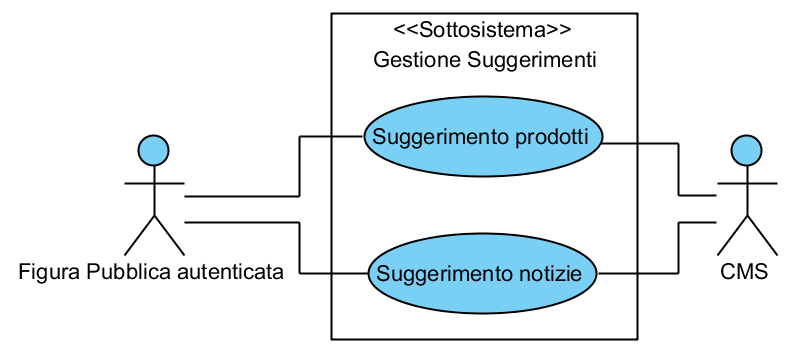
\includegraphics[width=\textwidth]{assets/visualParadigm/cu/GestioneSuggerimenti}
\end{center}
%***************  SUGGERIMENTO PRODOTTI *****************
%Accorpa suggerimento intelligente e simili
\cuTab{cu:suggerimentoProdotti}
{\getTitletodesc{att:figuraPubblicaAutenticata}}
{La persona connessa al sito è autenticata ed ha i privilegi di Figura Pubblica Autenticata. Il sistema sta mostrando alla persona la scheda di un prodotto}
{Il sistema sta mostrando alla persona una lista di \glspl{anteprima} di prodotti simili}
{\begin{enumCU}
	\item Il caso d'uso ha inizio quando una Figura Pubblica Autenticata richiede di mostrare le \glspl{anteprima} delle schede di prodotti simili a quella che sta visualizzando
	\item Il sistema mostra alla Figura Pubblica Autenticata una lista di \glspl{anteprima} di prodotti simili
\end{enumCU}}

\vspaceTab

%***************  SUGGERIMENTO NOTIZIE *****************
\cuTab{cu:notizieSimili}
{\getTitletodesc{att:figuraPubblicaAutenticata}}
{La persona connessa al sito è autenticata ed ha i privilegi di Figura Pubblica Autenticata. Il sistema sta mostrando alla persona la scheda di un prodotto}
{Il sistema sta mostrando alla persona una lista di \glspl{anteprima} di notizie simili}
{\begin{enumCU}
	\item Il caso d'uso ha inizio quando una Figura Pubblica Autenticata richiede di mostrare notizie simili alla notizia che sta visualizzando
	\item Il sistema mostra alla Figura Pubblica Autenticata una lista di \glspl{anteprima} di notizie simili
\end{enumCU}}

\subsection{Gestione account}
\begin{center}
   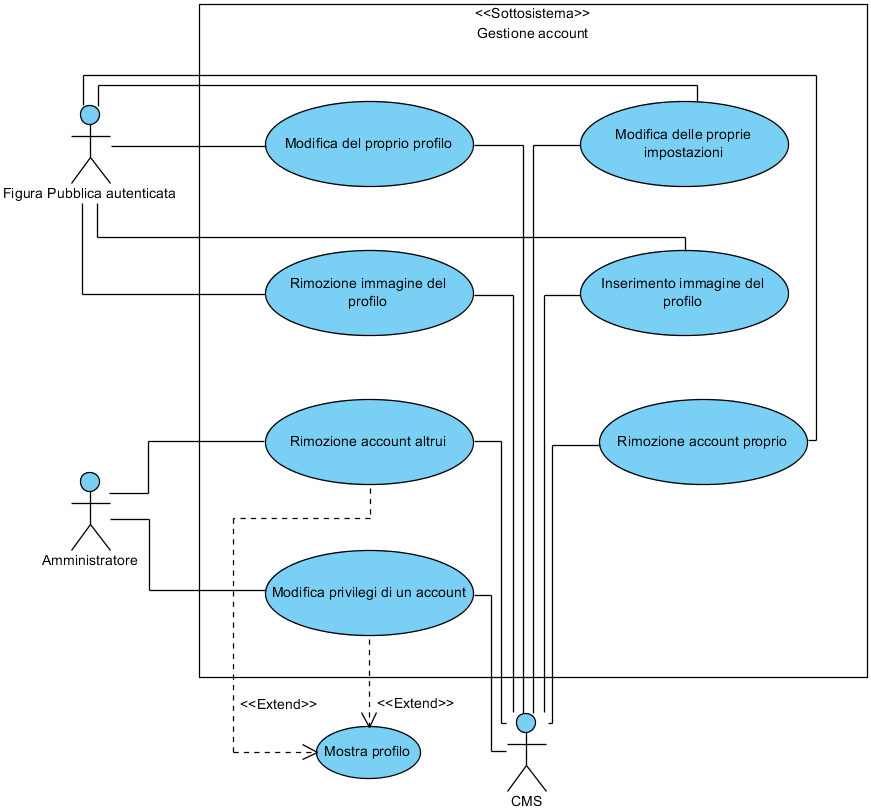
\includegraphics[width=\textwidth]{assets/visualParadigm/cu/GestioneAccount}
\end{center}
%***************  ACCESSO PROFILO *****************
\cuTab{cu:modificaProfilo}
{\getTitletodesc{att:figuraPubblicaAutenticata}, \getTitletodesc{att:figuraAmministrativa}}
{La persona connessa al sito è autenticata. Il sistema sta mostrando alla persona il suo profilo}
{Il profilo della persona è stato modificato}
{\begin{enumCU}
	\item Il caso d'uso ha inizio quando una persona autenticata nel sistema richiede di modificare il proprio profilo
	\item Il sistema mostra alla persona i campi modificabili
	\item La persona effettua le modifiche volute \label{modProf}
	\item La persona conferma le modifiche effettuate
	\item Il sistema memorizza le modifiche
\end{enumCU}}
%
\cuAlternativo{cu:modificaProfilo}
{Flusso alternativo 1}%
{Annulla modifica}%
{La persona connessa al sito è autenticata. Il sistema sta mostrando alla persona il suo profilo}
{\postNulle}%
{\begin{enumCU}
	\item Dopo il punto \ref{modProf} annulla le modifiche effettuate
\end{enumCU}}%

\vspaceTab

\cuTab{cu:inserisciImgProfilo}
{\getTitletodesc{att:figuraPubblicaAutenticata}, \getTitletodesc{att:figuraAmministrativa}}
{La persona connessa al sito è autenticata. Il sistema sta mostrando alla persona il suo profilo}
{Nel sistema è presente l'immagine del profilo della persona}
{\begin{enumCU}
	\item Il caso d'uso ha inizio quando una persona autenticata nel sistema richiede di inserire l'immagine del proprio profilo
	\item Il sistema richiede il percorso nel file system, o nella rete, dell'immagine da inserire 
	\item La persona inserisce il percorso dell'immagine nell'apposito campo\label{insimg1}
	\item La persona conferma il percorso dell'immagine inserito\label{insimg2}
	\item Il sistema scarica e memorizza l'immagine impostandola come immagine del profilo della persona
\end{enumCU}}
%
\cuAlternativo{cu:inserisciImgProfilo}
{Flusso alternativo 1}%
{Errore inserimento}%
{La persona connessa al sito è autenticata. Il sistema sta mostrando alla persona il suo profilo}
{\postNulle}%
{\begin{enumCU}
		\item Dopo il punto \ref{insimg2} il sistema non riesce a trovare, scaricare o inserire correttamente l'immagine
	\end{enumCU}}%
%
\cuAlternativo{cu:inserisciImgProfilo}
{Flusso alternativo 2}%
{Annulla inserimento}%
{La persona connessa al sito è autenticata. Il sistema sta mostrando alla persona il suo profilo}
{\postNulle}%
{\begin{enumCU}
		\item Dopo il punto \ref{insimg1} il produttore annulla l'inserimento dell'immagine
	\end{enumCU}}%

\vspaceTab

\cuTab{cu:rimuoviImgProfilo}
{\getTitletodesc{att:figuraPubblicaAutenticata}, \getTitletodesc{att:figuraAmministrativa}}
{La persona connessa al sito è autenticata. Il sistema sta mostrando alla persona il suo profilo. Nel sistema è presente l'immagine del profilo della persona}
{Nel sistema non è presente l'immagine del profilo della persona}
{\begin{enumCU}
	\item Il caso d'uso ha inizio quando una persona autenticata nel sistema richiede di rimuovere l'immagine del proprio profilo
	\item Il sistema richiede conferma della rimozione\label{annrimimg}
	\item La persona conferma la rimozione
	\item Il sistema rimuove l'immagine
\end{enumCU}}
%
\cuAlternativo{cu:rimuoviImgProfilo}
{Flusso alternativo 1}%
{Annulla rimozione}%
{La persona connessa al sito è autenticata. Il sistema sta mostrando alla persona il suo profilo. Nel sistema è presente l'immagine del profilo della persona}
{\postNulle}%
{\begin{enumCU}
		\item Dopo il punto \ref{annrimimg} la persona annulla l'operazione di rimozione
	\end{enumCU}}%

\vspaceTab

%***************  ACCESSO IMPOSTAZIONI *****************
\cuTab{cu:modificaImpostazioni}
{\getTitletodesc{att:figuraPubblicaAutenticata}, \getTitletodesc{att:figuraAmministrativa}}
{La persona connessa al sito è autenticata}
{Nel sistema le impostazioni della persona sono state modificate come richiesto}   
{\begin{enumCU}
	\item Il caso d'uso ha inizio quando una persona autenticata nel sistema richiede di modificare la pagina delle proprie impostazioni
	\item Il sistema mostra alla persona la pagina delle proprie impostazioni, abilitando solo i campi che la persona può modificare
	\item La persona modifica i campi presenti nella pagina\label{cumodimp:1}
	\item La persona conferma le modifiche effettuate 
	\item Il sistema memorizza le modifiche effettuate
\end{enumCU}
\ext{cu:rimozioneAccountProprio}}
%
\cuAlternativo{cu:modificaImpostazioni}
{Flusso alternativo 1}%
{Annulla modifica}%
{La persona connessa al sito è autenticata nel sistema}%
{\postNulle}%
{\begin{enumCU}
		\item Dopo il punto \ref{cumodimp:1} annulla le modifiche effettuate
	\end{enumCU}}%

\vspaceTab

%***************  RIMOZIONE ACCOUNT PROPRIO  *****************
\cuTab{cu:rimozioneAccountProprio}
{\getTitletodesc{att:figuraPubblicaAutenticata}}
{La persona connessa al sito è autenticata ed ha solo i privilegi di Figura Pubblica Autenticata}
{La persona non è più autenticata nel sistema. L'account della persona non è più presente nel sistema}
{\begin{enumCU}
	\item Il caso d'uso ha inizio quando una Figura Pubblica Autenticata nel sistema richiede di rimuovere il proprio account
	\item Il sistema chiede conferma della rimozione dell'account\label{curimaccprop:1}
	\item La persona conferma la rimozione
	\item Il sistema rimuove l'account del richiedente
\end{enumCU}}
%
\cuAlternativo{cu:rimozioneAccountProprio}
{Flusso alternativo 1}%
{Annulla rimozione}%
{La persona connessa al sito è autenticata ed ha solo i privilegi di Figura Pubblica Autenticata}%
{\postNulle}%
{\begin{enumCU}
		\item Dopo il punto \ref{curimaccprop:1} la persona annulla la rimozione dell'account
	\end{enumCU}}%

\vspaceTab

%***************  RIMOZIONE ACCOUNT ALTRUI  *****************
\cuTab{cu:rimozioneAccountAltrui}
{\getTitletodesc{att:amministratore}}
{La persona connessa al sito è autenticata e ha i privilegi di Amministratore. Il sistema sta mostrando alla persona un profilo associato ad un altro account}
{Nel sistema non è più presente l'account rimosso}
{\begin{enumCU}
	\item Il caso d'uso ha inizio quando un Amministratore richiede al sistema di rimuovere l'account associato al profilo che sta visualizzando
	\item Il sistema chiede conferma della rimozione dell'account\label{curimaccaltr:1}
	\item L'Amministratore conferma la rimozione
	\item Il sistema rimuove l'account selezionato
\end{enumCU}}
%
\cuAlternativo{cu:rimozioneAccountAltrui}
{Flusso alternativo 1}%
{Annulla rimozione}%
{La persona connessa al sito è autenticata e ha i privilegi di Amministratore. Il sistema sta mostrando alla persona un profilo associato ad un altro account}%
{\postNulle}%
{\begin{enumCU}
	\item Dopo il punto \ref{curimaccaltr:1} l'Amministratore annulla la rimozione dell'account
\end{enumCU}}%

\vspaceTab

%***************  Modifica privilegi  *****************
\cuTab{cu:modificaPrivilegiAccount}
{\getTitletodesc{att:amministratore}}
{La persona connessa al sito è autenticata e ha i privilegi di Amministratore. Il sistema sta mostrando alla persona una lista di \glspl{anteprima} di profili}
{Nel sistema sono stati aggiornati i privilegi di quell'account come richiesto}
{\begin{enumCU}
	\item Il caso d'uso ha inizio quando un Amministratore seleziona un'\gls{anteprima} profilo tra quelle mostrate nel risultato della ricerca e richiede di modificarne i privilegi
	\item Il sistema mostra all'Amministratore la lista dei privilegi, specificando quelli posseduti dall'account associato al profilo selezionato
	\item Il sistema chiede di modificare i privilegi posseduti dall'account
	\item L'Amministratore seleziona quali privilegi vuole fornire all'account\label{cufornpriv:1}
	\item L'Amministratore conferma la selezione
	\item Il sistema memorizza le scelte effettuate
\end{enumCU}}
%
\cuAlternativo{cu:modificaPrivilegiAccount}
{Flusso alternativo 1}%
{Annulla operazione}%
{La persona connessa al sito è autenticata e ha i privilegi di Amministratore. Il sistema sta mostrando alla persona una lista di \glspl{anteprima} di profili}%
{\postNulle}%
{\begin{enumCU}
		\item Dopo il punto \ref{cufornpriv:1} l'Amministratore annulla l'operazione
	\end{enumCU}}%

\vspaceTab

%***************  Gestione valutazioni *****************
\subsection{Gestione valutazioni}
\begin{center}
   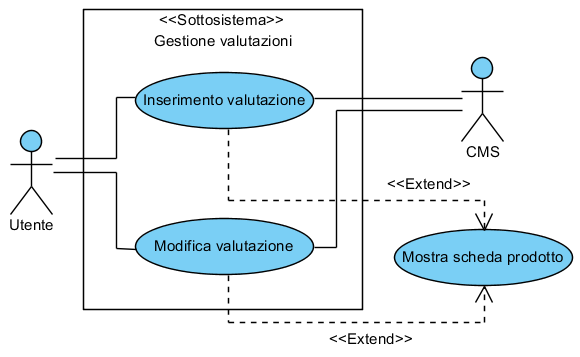
\includegraphics[width=\textwidth]{assets/visualParadigm/cu/GestioneValutazioni}
\end{center}
\cuTab{cu:inserisciValutazioneProdotto}
{\getTitletodesc{att:utente}}
{La persona connessa al sito è autenticata ed ha i privilegi di Utente. Il sistema sta mostrando alla persona la scheda di un prodotto che non ha già stato valutato}
{Nel sistema è stata aggiunta la valutazione della persona per il prodotto}
{\begin{enumCU}
	\item Il caso d'uso ha inizio quando un Utente richiede di effettuare la valutazione del prodotto che sta visualizzando
	\item Il sistema richiede all'Utente la valutazione per quel prodotto
	\item L'Utente inserisce la valutazione
	\item Il sistema memorizza la valutazione
\end{enumCU}
\ext{cu:inserisciRecensioneProdotto}
}


\vspaceTab

\cuTab{cu:modificaValutazioneProdotto}
{\getTitletodesc{att:utente}}
{La persona connessa al sito è autenticata ed ha i privilegi di Utente. Il sistema sta mostrando alla persona la scheda di un prodotto che ha già stato valutato}
{Nel sistema è stata modificata la valutazione del prodotto inserita dalla persona}
{\begin{enumCU}
	\item Il caso d'uso ha inizio quando un Utente richiede di modificare la valutazione del prodotto
	\item Il sistema mostra all'Utente la valutazione che ha effettuato per quel prodotto
	\item L'Utente inserisce la nuova valutazione
	\item Il sistema memorizza la nuova valutazione inserita
\end{enumCU}}

%***************  Gestione recensione *****************
\subsection{Gestione recensioni}
\begin{center}
   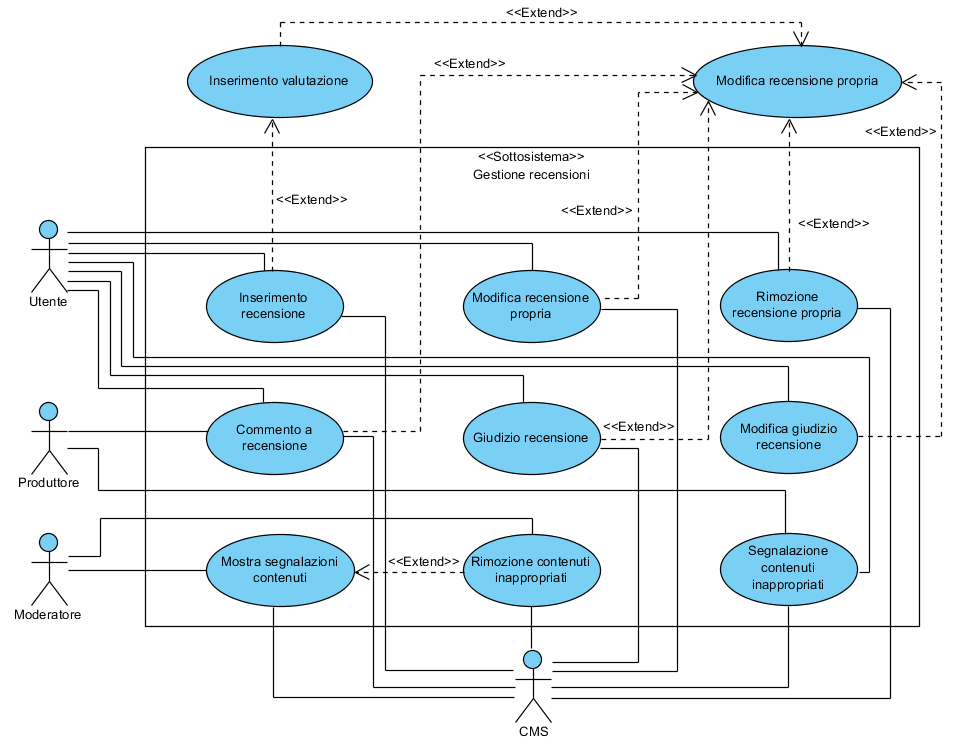
\includegraphics[width=\textwidth]{assets/visualParadigm/cu/GestioneRecensioni}
\end{center}
\cuTab{cu:inserisciRecensioneProdotto}
{\getTitletodesc{att:utente}}
{La persona connessa al sito è autenticata come Utente. Il sistema sta mostrando alla persona la scheda di un prodotto che ha già stato valutato}
{Nel sistema è presente la recensione dell'Utente per quel prodotto}
{\begin{enumCU}
	\item Il caso d'uso ha inizio quando un Utente richiede di effettuare la recensione del prodotto che sta visualizzando
	\item Il sistema richiede all'Utente il testo da inserire come recensione
	\item L'Utente inserisce la recensione\label{addrec:3}
	\item L'Utente conferma la recensione inserita
	\item Il sistema memorizza la recensione
\end{enumCU}}
%
\cuAlternativo{cu:inserisciRecensioneProdotto}
{Flusso alternativo 1}%
{Annulla inserimento}%
{La persona connessa al sito è autenticata come Utente. Il sistema sta mostrando alla persona la scheda di un prodotto che ha già stato valutato}%
{\postNulle}%
{\begin{enumCU}
		\item Dopo il punto \ref{addrec:3}, l'Utente annulla l'operazione di inserimento
	\end{enumCU}}%

\vspaceTab

\cuTab{cu:modificaRecensioneProdotto}
{\getTitletodesc{att:utente}}
{La persona connessa al sito è autenticata come Utente. Il sistema sta mostrando alla persona una recensione di un prodotto che ha effettuato}
{Nel sistema è stata modificata la recensione di quella persona per quel prodotto}
{\begin{enumCU}
	\item Il caso d'uso ha inizio quando un Utente richiede di modificare la recensione che sta visualizzando
	\item Il sistema mostra all'Utente la recensione che ha effettuato per quel prodotto
	\item L'Utente inserisce la nuova recensione \label{newrec:3}
	\item L'Utente conferma la nuova recensione inserita
	\item Il sistema memorizza la nuova recensione
\end{enumCU}}
%
\cuAlternativo{cu:modificaRecensioneProdotto}
{Flusso alternativo 1}%
{Annulla modifiche}%
{La persona connessa al sito è autenticata come Utente. Il sistema sta mostrando alla persona una recensione di un prodotto che ha effettuato}
{\postNulle}%
{\begin{enumCU}
		\item Dopo il punto \ref{newrec:3}, l'Utente annulla l'operazione di modifica
	\end{enumCU}}%

\vspaceTab

\cuTab{cu:eliminaRecensioneProdotto}
{\getTitletodesc{att:utente}}
{La persona connessa al sito è autenticata  come Utente. Il sistema sta mostrando alla persona una recensione di un prodotto che ha effettuato}
{Nel sistema è stata rimossa la recensione di quella persona}
{\begin{enumCU}
	\item Il caso d'uso ha inizio quando un Utente richiede di rimuovere la recensione per quel prodotto
	\item Il sistema mostra all'Utente la recensione che ha effettuato per quel prodotto
	\item Il sistema richiede di confermare la rimozione \label{remrec:3}
	\item L'Utente conferma la rimozione
	\item Il sistema rimuove la recensione
\end{enumCU}}
%
\cuAlternativo{cu:eliminaRecensioneProdotto}
{Flusso alternativo 1}%
{Annulla rimozione}%
{La persona connessa al sito è autenticata  come Utente. Il sistema sta mostrando alla persona una recensione di un prodotto effettuata dalla persona}
{\postNulle}%
{\begin{enumCU}
		\item Dopo il punto \ref{remrec:3}, l'Utente annulla l'operazione di rimozione
	\end{enumCU}}%

\vspaceTab

\cuTab{cu:commentoRecensione}
{\getTitletodesc{att:figuraPubblicaAutenticata}}
{La persona è connessa al sito ed ha i privilegi di Figura Pubblica Autenticata. Il sistema sta mostrando alla persona la recensione di un prodotto}
{Nel sistema è presente il commento inserito dalla persona per quella recensione}
{\begin{enumCU}
	\item Il caso d'uso ha inizio quando la persona richiede di effettuare un commento alla recensione che sta visualizzando\label{commrifiutato2}
	\item Il sistema richiede di inserire un nuovo commento 
	\item La persona inserisce il commento\label{addcom:3}
	\item La persona conferma il commento inserito
	\item Il sistema memorizza il commento
\end{enumCU}}
%
\cuAlternativo{cu:commentoRecensione}
{Flusso alternativo 1}%
{Annulla rimozione}%
{La persona è connessa al sito ed ha i privilegi di Figura Pubblica Autenticata. Il sistema sta mostrando alla persona la recensione di un prodotto}
{\postNulle}%
{\begin{enumCU}
		\item Dopo il punto \ref{addcom:3}, la persona annulla l'operazione di inserimento
	\end{enumCU}}%
%
\cuAlternativo{cu:commentoRecensione}
{Flusso alternativo 2}%
{Errore inserimento}%
{La persona è connessa al sito ed ha i privilegi di Produttore. Il sistema sta mostrando alla persona la recensione di un prodotto}
{\postNulle}%
{\begin{enumCU}
		\item Nel punto \ref{commrifiutato2} la persona richiede di effettuare un commento alla recensione che sta visualizzando, di un prodotto non suo
		\item Dopo il punto \ref{commrifiutato2} il sistema rifiuta la richiesta
	\end{enumCU}}%

\vspaceTab

\cuTab{cu:giudizioRecensione}
{\getTitletodesc{att:utente}}
{La persona connessa al sito è autenticata come Utente. Il sistema sta mostrando alla persona la recensione di un prodotto che non ha giudicato}
{Nel sistema è presente il giudizio di quella persona per quella recensione}
{\begin{enumCU}
	\item Il caso d'uso ha inizio quando un Utente richiede di esprimere un giudizio (positivo o negativo) sulla recensione che sta visualizzando
	\item Il sistema mostra all'Utente la recensione
	\item Il sistema richiede all'Utente il giudizio per quella recensione
	\item L'Utente inserisce il giudizio
	\item Il sistema memorizza il giudizio
\end{enumCU}}


\cuTab{cu:modificaGiudizioRecensione}
{\getTitletodesc{att:utente}}
{La persona connessa al sito è autenticata  come Utente. Il sistema sta mostrando alla persona la recensione di un prodotto che ha già giudicato}
{Nel sistema è stato modificato il giudizio di quella persona per quella recensione}
{\begin{enumCU}
	\item Il caso d'uso ha inizio quando un Utente richiede di modificare un giudizio della recensione che sta visualizzando
	\item Il sistema mostra all'Utente la recensione
	\item Il sistema mostra all'Utente il suo giudizio per quella recensione
	\item Il sistema richiede all'Utente il nuovo giudizio per quella recensione
	\item L'Utente inserisce il nuovo giudizio
	\item Il sistema memorizza il nuovo giudizio
\end{enumCU}}

\vspaceTab

\cuTab{cu:segnalazioneContenutiInap}
{\getTitletodesc{att:figuraPubblicaAutenticata}}
{La persona è connessa al sito ed ha i privilegi di Figura Pubblica Autenticata. Il sistema sta mostrando alla persona un \gls{contenuto}}
{Nel sistema è presente la segnalazione di quella persona per quel \gls{contenuto}}
{\begin{enumCU}
	\item Il caso d'uso ha inizio quando una persona richiede di segnalare il \gls{contenuto} che sta visualizzando in quanto inappropriato
	\item Il sistema richiede alla persona di specificare il motivo della segnalazione
	\item La persona inserisce il motivo della segnalazione\label{annullasegn}
	\item La persona conferma la segnalazione
	\item Il sistema memorizza la segnalazione allegando un \gls{riferimento} al \gls{contenuto} segnalato
\end{enumCU}}
%
\cuAlternativo{cu:segnalazioneContenutiInap}
{Flusso alternativo 1}%
{Annulla segnalazione}%
{La persona è connessa al sito ed ha i privilegi di Figura Pubblica Autenticata. Il sistema sta mostrando alla persona un \gls{contenuto}}
{\postNulle}%
{\begin{enumCU}
		\item Dopo il punto \ref{annullasegn}, la persona annulla l'operazione di segnalazione
	\end{enumCU}}%

\vspaceTab

\cuTab{cu:mostraSegnContenutiInap}
{\getTitletodesc{att:moderatore}}
{La persona connessa al sito è autenticata  ed ha i privilegi di Moderatore. Nel sistema è presente almeno una segnalazione}
{Il sistema sta mostrando alla persona il \gls{contenuto} segnalato}
{\begin{enumCU}
	\item Il caso d'uso ha inizio quando un Moderatore richiede di visualizzare una segnalazione
	\item Il sistema mostra al Moderatore le segnalazioni presenti nel sistema\label{delsegn:3}
	\item Il Moderatore seleziona una segnalazione tra quelle proposte
	\item Il sistema mostra la segnalazione \label{delsegn:4}
	\item Il Moderatore richiede di visualizzare il \gls{contenuto} segnalato
	\item Il sistema mostra il \gls{contenuto} segnalato
\end{enumCU}
\ext{cu:rimozioneContenutiInap}
}
%
\cuAlternativo{cu:mostraSegnContenutiInap}
{Flusso alternativo 1}%
{Elimina segnalazione}%
{La persona connessa al sito è autenticata  ed ha i privilegi di Moderatore. Nel sistema è presente almeno una segnalazione}
{Nel sistema non è più presente quella segnalazione}%
{\begin{enumCU}
		\item Dopo il punto \ref{delsegn:4}, il Moderatore elimina la segnalazione
\end{enumCU}}%
%marcare segnalazione come risolta/eliminarla dalla lista
%	
\cuAlternativo{cu:mostraSegnContenutiInap}
{Flusso alternativo 2}%
{Annulla operazione di selezione}%
{La persona connessa al sito è autenticata ed ha i privilegi di Moderatore. Nel sistema è presente almeno una segnalazione}%
{\postNulle}%
{\begin{enumCU}
		\item Dopo il punto \ref{delsegn:3} la persona annulla l'operazione di selezione
\end{enumCU}}%

\vspaceTab

\cuTab{cu:rimozioneContenutiInap}
{\getTitletodesc{att:moderatore}}
{La persona connessa al sito è autenticata ed ha i privilegi di Moderatore. Il sistema sta mostrando alla persona un \gls{contenuto}}
{Nel sistema non è più presente il \gls{contenuto}}
{\begin{enumCU}
	\item Il caso d'uso ha inizio quando un Moderatore richiede di rimuovere il \gls{contenuto} che sta visualizzando\label{rim2}
	\item Il sistema richiede al Moderatore di confermare la rimozione\label{delcont:3}
	\item Il Moderatore conferma la rimozione 
	\item Il sistema rimuove il \gls{contenuto} inappropriato
\end{enumCU}}
%
\cuAlternativo{cu:rimozioneContenutiInap}
{Flusso alternativo 1}%
{Annulla rimozione}%
{La persona connessa al sito è autenticata ed ha i privilegi di Moderatore. Il sistema sta mostrando alla persona un \gls{contenuto}}
{\postNulle}%
{\begin{enumCU}
		\item Dopo il punto \ref{delcont:3}, il Moderatore annulla l'operazione di rimozione
\end{enumCU}}%


\subsection{Interazione tra figure}
\begin{center}
   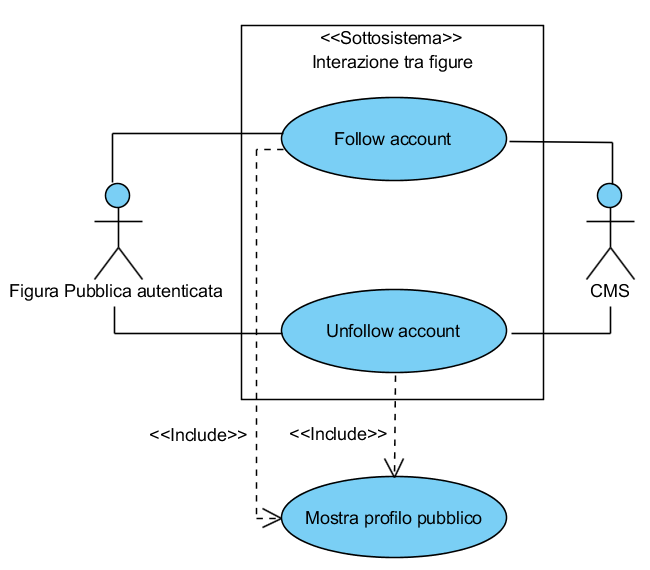
\includegraphics[width=\textwidth]{assets/visualParadigm/cu/InterazioneTraFigure}
\end{center}
%****************** FOLLOW ACCOUNT ***********
\cuTab{cu:followAccount}
{\getTitletodesc{att:figuraPubblicaAutenticata}}
{La persona è connessa al sito ed ha i privilegi di Figura Pubblica Autenticata. Il sistema sta mostrando alla persona un profilo associato ad un altro account}
{La persona segue quell'account}
{\begin{enumCU}
	\item Il caso d'uso ha inizio quando la persona richiede di seguire l'account associato al profilo visualizzato
	\item Il sistema accetta l`operazione
\end{enumCU}}

\vspaceTab

%****************** UNFOLLOW ACCOUNT ***********
\cuTab{cu:unFollowAccount}
{\getTitletodesc{att:figuraPubblicaAutenticata}}
{La persona è connessa al sito ed ha i privilegi di Figura Pubblica Autenticata. Il sistema sta mostrando alla persona un profilo associato ad un account che segue}
{La persona non segue più quell'account}
{\begin{enumCU}
	\item Il caso d'uso ha inizio quando la persona richiede di non seguire più l'account associato a quel profilo
	\item Il sistema accetta l`operazione
\end{enumCU}}

\subsection{Gestione ticket}
\begin{center}
   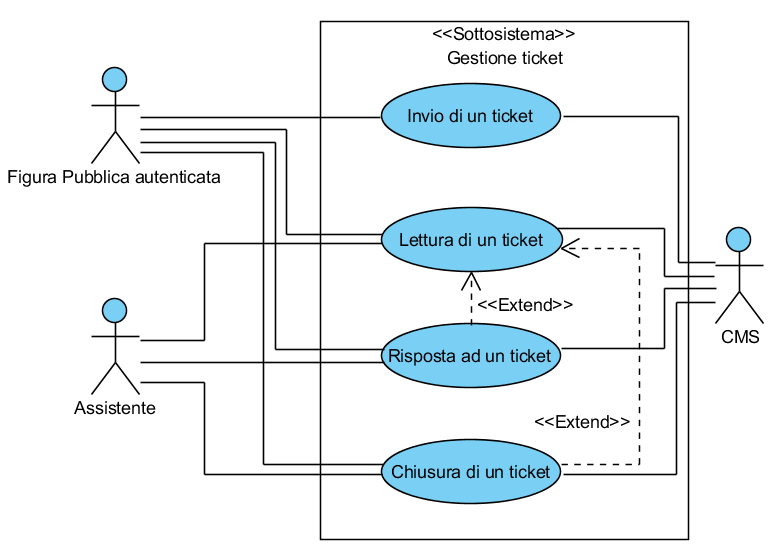
\includegraphics[width=\textwidth]{assets/visualParadigm/cu/GestioneTicket}
\end{center}
%****************** INVIO TICKET ***********
\cuTab{cu:ticketInvio}
{\getTitletodesc{att:figuraPubblicaAutenticata}}
{La persona è connessa al sito ed ha i privilegi di Figura Pubblica Autenticata}
{Nel sistema è presente il ticket creato da quella persona}
{\begin{enumCU}
	\item Il caso d'uso ha inizio quando la persona richiede la creazione di un ticket per ricevere assistenza
	\item Il sistema richiede di compilare la scheda necessaria alla creazione del ticket
	\item La persona compila la scheda\label{cucretick:1}
	\item La persona conferma i dati inseriti
	\item Il sistema memorizza il ticket
\end{enumCU}}
%
\cuAlternativo{cu:ticketInvio}
{Flusso alternativo 1}%
{Annulla creazione ticket}%
{La persona è connessa al sito ed ha i privilegi di Figura Pubblica Autenticata}%
{\postNulle}%
{\begin{enumCU}
		\item Dopo il punto \ref{cucretick:1} la persona annulla la creazione del ticket
	\end{enumCU}}%

\vspaceTab

%****************** RISPOSTA TICKET ***********
\cuTab{cu:ticketRisposta}
{\getTitletodesc{att:figuraPubblicaAutenticata}, \getTitletodesc{att:assistente}}
{La persona è connessa al sito ed ha i privilegi di Assistente, oppure ha i privilegi di Figura Pubblica Autenticata. Il sistema sta mostrando alla persona un ticket. Se la persona è una Figura Pubblica Autenticata deve essere il creatore del ticket mostrato}
{Nel sistema è presente la risposta al ticket in questione}
{\begin{enumCU}
	\item Il caso d'uso ha inizio quando la persona richiede di rispondere a quel ticket
	\item Il sistema richiede di compilare la scheda necessaria alla creazione della risposta
	\item La persona compila la scheda necessaria all'inserimento della risposta\label{curisptick:1}
	\item La persona conferma i dati inseriti
	\item Il sistema memorizza la risposta al ticket
\end{enumCU}}
%
\cuAlternativo{cu:ticketRisposta}
{Flusso alternativo 1}%
{Annulla risposta ticket}%
{La persona è connessa al sito ed ha i privilegi di Assistente, oppure ha i privilegi di Figura Pubblica Autenticata. Il sistema sta mostrando alla persona un ticket. Se la persona è una Figura Pubblica Autenticata deve essere il creatore del ticket mostrato}%
{\postNulle}%
{\begin{enumCU}
		\item Dopo il punto \ref{curisptick:1} la persona annulla l'inserimento della risposta
	\end{enumCU}}%

\vspaceTab

%****************** CHIUDI TICKET ***********
\cuTab{cu:ticketChiudi}
{\getTitletodesc{att:figuraPubblicaAutenticata}, \getTitletodesc{att:assistente}}
{La persona è connessa al sito ed ha i privilegi di Assistente, oppure ha i privilegi di Figura Pubblica Autenticata. Il sistema sta mostrando alla persona un ticket. Se la persona è una Figura Pubblica Autenticata deve essere il creatore del ticket mostrato}
{Il ticket in questione risulta chiuso nel sistema}
{\begin{enumCU}
	\item Il caso d'uso ha inizio quando la persona richiede di chiudere il ticket\label{cuchiutick:0}
	\item Il sistema richiede conferma della chiusura\label{cuchiutick:1}
	\item La persona conferma la chiusura del ticket
	\item Il sistema accetta l'operazione e memorizza il ticket come chiuso
\end{enumCU}}
%
\cuAlternativo{cu:ticketChiudi}
{Flusso alternativo 1}%
{Annulla chiusura ticket}%
{La persona è connessa al sito ed ha i privilegi di Assistente, oppure ha i privilegi di Figura Pubblica Autenticata. Il sistema sta mostrando alla persona un ticket. Se la persona è una Figura Pubblica Autenticata deve essere il creatore del ticket mostrato}%
{\postNulle}%
{\begin{enumCU}
		\item Dopo il punto \ref{cuchiutick:1} la persona annulla l'operazione di chiusura
	\end{enumCU}}%

\vspaceTab

%****************** LEGGI TICKET ***********
\cuTab{cu:ticketLettura}
{\getTitletodesc{att:figuraPubblicaAutenticata}, \getTitletodesc{att:assistente}}
{La persona è connessa al sito ed ha i privilegi di Assistente, oppure ha i privilegi di Figura Pubblica Autenticata ed è il creatore di un ticket}
{Il sistema sta mostrando alla persona il ticket}
{\begin{enumCU}
	\item Il caso d'uso ha inizio quando la persona richiede di visualizzare un ticket
	\item Il sistema mostra alla persona i ticket a cui ha accesso\label{annsel}
	\item La persona seleziona un ticket
	\item Il sistema mostra il ticket alla persona
\end{enumCU}
\ext{cu:ticketRisposta}
\ext{cu:ticketChiudi}
}
%	
\cuAlternativo{cu:ticketLettura}
{Flusso alternativo 1}%
{Annulla operazione di selezione}%
{La persona è connessa al sito ed ha i privilegi di Assistente, oppure ha i privilegi di Figura Pubblica Autenticata ed è il creatore di un ticket}%
{\postNulle}%
{\begin{enumCU}
		\item Dopo il punto \ref{annsel} la persona annulla l'operazione di selezione
\end{enumCU}}%


\subsection{Ricerca contenuti}
\begin{center}
   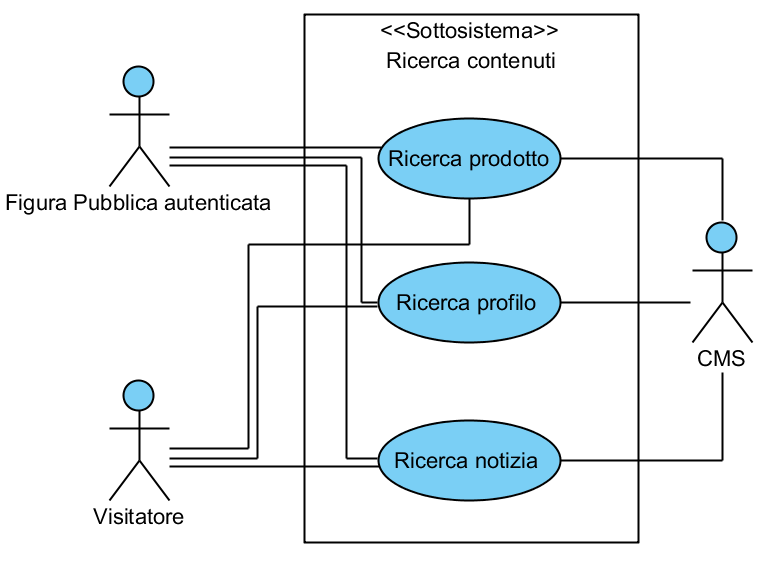
\includegraphics[width=\textwidth]{assets/visualParadigm/cu/RicercaContenuti}
\end{center}
%****************** RICERCA PRODOTTO ***********
\cuTab{cu:ricercaProdotto}
{\getTitletodesc{att:visitatore}, \getTitletodesc{att:figuraPubblicaAutenticata}}
{La persona è connessa al sito}
{Il sistema sta mostrando alla persona la lista delle \glspl{anteprima} delle schede dei prodotti cercati}
{\begin{enumCU}
	\item Il caso d'uso ha inizio quando la persona richiede di effettuare la ricerca della scheda di un prodotto
	\item Il sistema richiede di complilare la scheda necessaria per definire i parametri di ricerca
	\item La persona inserisce i dati negli appositi campi \label{curicprod:1}
	\item La persona conferma i dati inseriti
	\item Il sistema effettua la ricerca richiesta
	\item Il sistema mostra le \glspl{anteprima} dei risultati della ricerca
\end{enumCU}
\ext{cu:mostraProdotto}
}
%
\cuAlternativo{cu:ricercaProdotto}
{Flusso alternativo 1}%
{Annulla ricerca}%
{La persona è connessa al sito}%
{\postNulle}%
{\begin{enumCU}
		\item Dopo il punto \ref{curicprod:1} la persona annulla la ricerca
	\end{enumCU}}%

\vspaceTab

%****************** RICERCA PROFILO ***********
\cuTab{cu:ricercaProfilo}
{\getTitletodesc{att:visitatore}, \getTitletodesc{att:figuraPubblicaAutenticata}}
{La persona è connessa al sito}
{Il sistema sta mostrando alla persona la lista delle \glspl{anteprima} dei profili cercati}
{\begin{enumCU}
	\item Il caso d'uso ha inizio quando la persona richiede di effettuare la ricerca di un profilo
	\item Il sistema richiede di complilare la scheda necessaria per definire i parametri di ricerca
	\item La persona inserisce i dati negli appositi campi \label{curicprof:1}
	\item La persona conferma i dati inseriti
	\item Il sistema effettua la ricerca richiesta
	\item Il sistema mostra le aneteprime dei risultati della ricerca
\end{enumCU}
\ext{cu:mostraVetrina}
\ext{cu:mostraProfilo}
}
%
\cuAlternativo{cu:ricercaProfilo}
{Flusso alternativo 1}%
{Annulla ricerca}%
{La persona è connessa al sito}%
{\postNulle}%
{\begin{enumCU}
		\item Dopo il punto \ref{curicprof:1} la persona annulla la ricerca
	\end{enumCU}}%

\vspaceTab


%****************** RICERCA NOTIZIA ***********
\cuTab{cu:ricercaNotizia}
{\getTitletodesc{att:visitatore}, \getTitletodesc{att:figuraPubblicaAutenticata}}
{La persona è connessa al sito}
{Il sistema sta mostrando alla persona la lista delle \glspl{anteprima} delle notizie cercati}
{\begin{enumCU}
	\item Il caso d'uso ha inizio quando la persona richiede di effettuare la ricerca di una notizia
	\item Il sistema richiede di compilare la scheda necessaria per definire i parametri di ricerca
	\item La persona inserisce i dati negli appositi campi \label{curicnot:1}
	\item La persona conferma i dati inseriti
	\item Il sistema effettua la ricerca richiesta
	\item Il sistema mostra le \glspl{anteprima} dei risultati della ricerca
\end{enumCU}
\ext{cu:mostraNotizia}
}
%
\cuAlternativo{cu:ricercaNotizia}
{Flusso alternativo 1}%
{Annulla ricerca}%
{La persona è connessa al sito}%
{\postNulle}%
{\begin{enumCU}
		\item Dopo il punto \ref{curicnot:1} la persona annulla la ricerca
	\end{enumCU}}%


\subsection{Gestione prodotti mancanti}
\begin{center}
   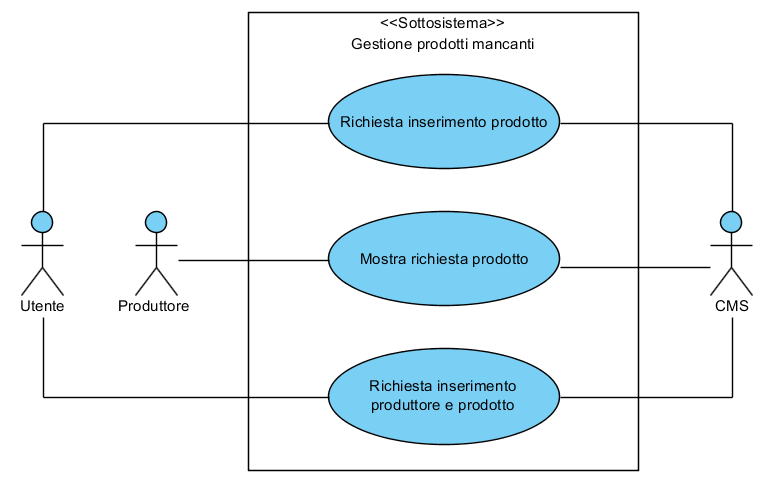
\includegraphics[width=\textwidth]{assets/visualParadigm/cu/GestioneProdottiMancanti}
\end{center}
%****************** RICHIESTA PRODOTTO ***********
\cuTab{cu:richiestaInsProdotto}
{\getTitletodesc{att:utente}}
{La persona connessa al sito è autenticata come Utente. Il sistema sta mostrando alla persona la vetrina di un Produttore}
{Il sistema contiene la richiesta di inserimento della scheda del prodotto creata, indirizzata al Produttore}
{\begin{enumCU}
		\item Il caso d'uso ha inizio quando un Utente richiede al Produttore, proprietario della vetrina che sta visualizzando, di inserire una sua scheda prodotto non già presente
		\item Il sistema richiede di compilare una scheda provvisoria del prodotto da inserire
		\item L'Utente inserisce i dati richiesti\label{curicinsimmpro:1}
		\item L'Utente conferma i dati inseriti 
		\item Il sistema richiede zero o più percorsi nel file system, o nella rete, delle immagini del prodotto da inserire
		\item L'Utente inserisce nell'apposito campo zero o più percorsi delle immagini che vuole inserire\label{curicinsimmpro:2}
		\item L'Utente conferma i percorsi inseriti\label{curicinsimmpro:3}
		\item Il sistema memorizza i dati inseriti, i percorsi inseriti e carica le immagini nel sistema
		\item Il sistema crea una nuova richiesta di inserimento prodotto per il Produttore
	\end{enumCU}}
%
\cuAlternativo{cu:richiestaInsProdotto}
{Flusso alternativo 1}%
{Annulla richiesta}%
{La persona connessa al sito è autenticata come Utente. Il sistema sta mostrando alla persona la vetrina di un Produttore}%
{\postNulle}%
{\begin{enumCU}
		\item Dopo il punto \ref{curicinsimmpro:2} o dopo il punto \ref{curicinsimmpro:1} l'Utente annulla la richiesta
	\end{enumCU}}%
%
\cuAlternativo{cu:richiestaInsProdotto}
{Flusso alternativo 2}%
{Errore richiesta}%
{La persona connessa al sito è autenticata come Utente. Il sistema sta mostrando alla persona la vetrina di un Produttore}%
{\postNulle}%
{\begin{enumCU}
		\item Dopo il punto \ref{curicinsimmpro:3} il sistema non riesce a trovare, caricare o inserire correttamente una o più immagini
	\end{enumCU}}%

\vspaceTab

\cuTab{cu:mostraRichiestaInsProdotto}
{\getTitletodesc{att:produttore}}
{La persona connessa al sito è autenticata come Produttore. Nel sistema è presente una richiesta di inserimento prodotto a lei indirizzata}
{Nella vetrina del Produttore è presente la scheda del prodotto suggerito}
{\begin{enumCU}
		\item Il caso d'uso ha inizio quando un Produttore richiedere di visualizzare le proprie richieste di aggiunta di schede prodotto in sospeso
		\item Il sistema richiede di selezionare quale richiesta visualizzare
		\item Il Produttore seleziona una richiesta
		\item Il sistema mostra al Produttore la scheda provvisoria del prodotto compilata dall'Utente che ha effettuato la richiesta \label{cuvisricprodel}
		\item Il Produttore modifica i campi nella scheda o inserisce quelli mancanti \label{cuvisricpro:1}
		\item Il Produttore conferma i dati inseriti
		\item Il sistema richiede zero o più percorsi nel file system, o nella rete, delle immagini del prodotto da inserire
		\item Il Produttore inserisce nell'apposito campo uno (zero se già inserite dall'utente) o più percorsi delle immagini che vuole inserire \label{cuvisricpro:2}
		\item Il Produttore conferma i percorsi inseriti \label{cuvisricpro:3}
		\item Il sistema memorizza i dati inseriti, i percorsi inseriti e carica le immagini nel sistema
	\end{enumCU}}
%
\cuAlternativo{cu:mostraRichiestaInsProdotto}
{Flusso alternativo 1}%
{Elimina richiesta}%
{La persona connessa al sito è autenticata come Produttore. Nel sistema è presente una richiesta di inserimento prodotto a lei indirizzata}
{Nel sistema non è più presente la richiesta}%
{\begin{enumCU}
		\item Dopo il punto \ref{cuvisricprodel} il Produttore richede di eliminare la richiesta
		\item Il sistema accetta l'operazione e rimuove la richiesta
	\end{enumCU}}%
%
\cuAlternativo{cu:mostraRichiestaInsProdotto}
{Flusso alternativo 2}%
{Annulla inserimento}%
{La persona connessa al sito è autenticata come Produttore. Nel sistema è presente una richiesta di inserimento prodotto a lei indirizzata}
{\postNulle}%
{\begin{enumCU}
		\item Dopo il punto \ref{cuvisricpro:2} o dopo il punto \ref{cuvisricpro:1} il Produttore annulla l'inserimento
	\end{enumCU}}%
%
\cuAlternativo{cu:mostraRichiestaInsProdotto}
{Flusso alternativo 3}%
{Errore inserimento}%
{La persona connessa al sito è autenticata come Produttore. Nel sistema è presente una richiesta di inserimento prodotto a lei indirizzata}
{\postNulle}%
{\begin{enumCU}
		\item Dopo il punto \ref{cuvisricpro:3} il sistema non riesce a trovare, caricare o inserire correttamente una o più immagini
	\end{enumCU}}%

\vspaceTab

\cuTab{cu:richiestaInsProduttore}
{\getTitletodesc{att:utente}}
{La persona connessa al sito è autenticata come Utente}
{Nel sistema è presente il ticket creato}
{\begin{enumCU}
		\item Il caso d'uso ha inizio quando un Utente richiede di inserire la scheda di un prodotto mancante di un Produttore non presente nel sistema
		\item Il sistema richiede di compilare una scheda provvisoria del prodotto da inserire
		\item L'Utente inserisce i dati richiesti \label{cuinsproduttore:1}
		\item L'Utente conferma i dati inseriti 
		\item Il sistema richiede zero o più percorsi nel file system, o nella rete, delle immagini del prodotto da inserire
		\item L'Utente inserisce nell'apposito campo zero o più percorsi delle immagini che vuole inserire \label{cuinsproduttore:2}
		\item L'Utente conferma i percorsi inseriti \label{cuinsproduttore:3}
		\item Il sistema memorizza i dati inseriti, i percorsi inseriti e salva le immagini nel sistema
		\item Il sistema richiede di compilare un profilo provvisorio, con almeno un nome e un recapito, del produttore
		\item L'Utente inserisce i dati richiesti \label{cuinsproduttore:0}
		\item L'Utente conferma i dati inseriti
		\item Il sistema crea un ticket allegando i riferimenti alle schede compilate
	\end{enumCU}}
%
\cuAlternativo{cu:richiestaInsProduttore}
{Flusso alternativo 1}%
{Annulla inserimento}%
{La persona connessa al sito è autenticata come Utente}%
{\postNulle}%
{\begin{enumCU}
		\item Dopo il punto \ref{cuinsproduttore:1}, il punto \ref{cuinsproduttore:2} o dopo il punto \ref{cuinsproduttore:0} l'Utente annulla l'operazione
	\end{enumCU}}%
%
\cuAlternativo{cu:richiestaInsProduttore}
{Flusso alternativo 2}%
{Errore inserimento}%
{La persona connessa al sito è autenticata come Utente}%
{\postNulle}%
{\begin{enumCU}
		\item Dopo il punto \ref{cuinsproduttore:3} il sistema non riesce a trovare, caricare o inserire correttamente una o più immagini
	\end{enumCU}}%

\subsection{Visualizzazione contenuti pubblici}
\begin{center}
   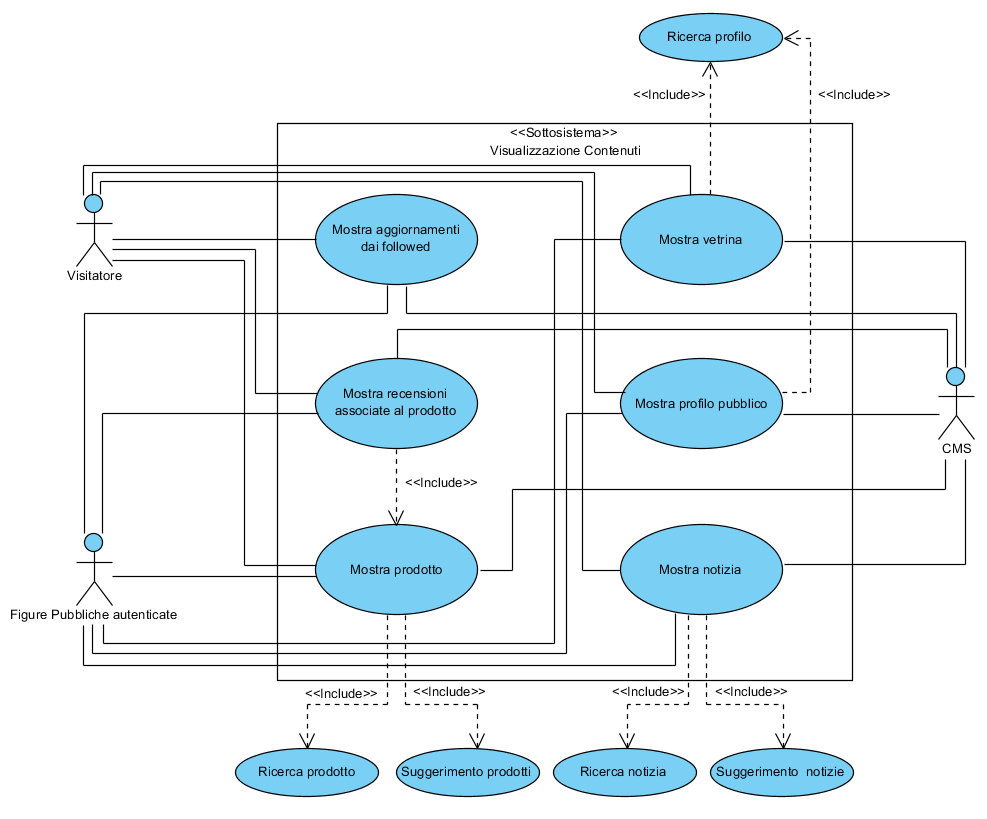
\includegraphics[width=\textwidth]{assets/visualParadigm/cu/Visualizzazione}
\end{center}
%accorpa visalizza prodotti in vetrina e visualizza vetrina
\cuTab{cu:mostraVetrina}
{\getTitletodesc{att:visitatore}, \getTitletodesc{att:figuraPubblicaAutenticata}}
{La persona è connessa al sito. Il sistema sta mostrando alla persona una lista di \glspl{anteprima} di profili di Produttori}
{Il sistema sta mostrando alla persona la vetrina del Produttore selezionato}
{\begin{enumCU}
	\item Il caso d'uso ha inizio quando una persona seleziona un \gls{anteprima} fra quelle presenti nella lista di \glspl{anteprima} di profili che sta visualizzando\label{cu:mostraVetr1}
	\item Il sistema mostra alla persona la vetrina del Produttore selezionato
\end{enumCU}
\ext{cu:statistichePrivateVetrina}
\ext{cu:personalizzaVetrinaInsProd}
\ext{cu:personalizzaVetrinaInsImg}
\ext{cu:personalizzaVetrinaDelImg}
\ext{cu:personalizzaVetrinaInsDesc}
\ext{cu:personalizzaVetrinaModDesc}
\ext{cu:richiestaInsProdotto}
}
%
\cuAlternativo{cu:mostraVetrina}%
{Flusso alternativo 1}%
{Selezione alternativa}%
{La persona è connessa al sito}%
{Il sistema sta mostrando alla persona la vetrina selezionata}%
{\begin{enumCU}
	\item Non viene effettuato il punto \ref{cu:mostraVetr1}, ma la persona seleziona un \gls{riferimento} verso una vetrina
\end{enumCU}}%
%
\cuAlternativo{cu:mostraVetrina}%
{Flusso alternativo 2}%
{Errore ricerca}%
{La persona è connessa al sito. Il sistema sta mostrando alla persona una lista di \glspl{anteprima} di profili}%
{\postNulle}%
{\begin{enumCU}
	\item Dopo il passo \ref{cu:mostraVetr1}, non ci sono risultati per la ricerca effettuata
	\item Il sistema visualizza un avvertimento e torna al passo \ref{cu:mostraVetr1}
\end{enumCU}}%

\vspaceTab

\cuTab{cu:mostraProdotto}{\getTitletodesc{att:visitatore}, \getTitletodesc{att:figuraPubblicaAutenticata}}
{La persona è connessa al sito. Il sistema sta mostrando alla persona una lista di \glspl{anteprima} di schede di prodotti}
{Il sistema sta mostrando alla persona la scheda del prodotto selezionato}
{\begin{enumCU}
	\item Il caso d'uso ha inizio quando una persona seleziona un \gls{anteprima} fra quelle presenti nella lista di \glspl{anteprima} prodotto che sta visualizzando\label{cu:mostraProd1}
	\item Il sistema mostra alla persona il prodotto selezionato
	\item \inc{cu:suggerimentoProdotti}
\end{enumCU}
\ext{cu:personalizzaVetrinaModProd}
\ext{cu:inserisciValutazioneProdotto}
\ext{cu:modificaValutazioneProdotto}
\ext{cu:mostraRecensioniProdotto}
}
%
\cuAlternativo{cu:mostraProdotto}
{Flusso alternativo 1}%
{Selezione alternativa}%
{La persona è connessa al sito}%
{Il sistema sta mostrando alla persona la scheda del prodotto selezionato}%
{\begin{enumCU}
		\item Non viene effettuato il punto \ref{cu:mostraProd1}, ma la persona seleziona un \gls{riferimento} verso la scheda di un prodotto
\end{enumCU}}%
%
\cuAlternativo{cu:mostraProdotto}
{Flusso alternativo 2}%
{Errore ricerca}%
{La persona è connessa al sito. Il sistema sta mostrando alla persona una lista di \glspl{anteprima} di schede di prodotti}%
{\postNulle}%
{\begin{enumCU}
		\item Dopo il passo \ref{cu:mostraProd1}, non ci sono risultati per la ricerca effettuata
		\item Il sistema visualizza un avvertimento e torna al passo \ref{cu:mostraProd1}
\end{enumCU}}%

\vspaceTab

\cuTab{cu:mostraRecensioniProdotto}
{\getTitletodesc{att:visitatore}, \getTitletodesc{att:figuraPubblicaAutenticata}}
{La persona è connessa al sito. Il sistema sta mostrando alla persona la scheda di un prodotto}
{Il sistema sta mostrando alla persona le recensioni associate al prodotto}
{\begin{enumCU}
	\item Il caso d'uso ha inizio quando una persona richiede di visualizzare le recensioni della scheda prodotto che sta visualizzando\label{cu:mostraRec1}
	\item Il sistema mostra alla persona le recensioni relative a quel prodotto
\end{enumCU}
\ext{cu:mostraRecensione}
}
%
\cuAlternativo{cu:mostraRecensioniProdotto}
{Flusso alternativo 1}%
{Recensioni assenti}%
{La persona è connessa al sito. Il sistema sta mostrando alla persona la scheda di un prodotto}%
{\postNulle}%
{\begin{enumCU}
		\item Dopo il passo \ref{cu:mostraRec1}, non ci sono risultati per la ricerca effettuata
		\item Il sistema mostra un avvertimento e annulla l'operazione
\end{enumCU}}

\vspaceTab

\cuTab{cu:mostraRecensione}
{\getTitletodesc{att:visitatore}, \getTitletodesc{att:figuraPubblicaAutenticata}}
{La persona è connessa al sito. Il sistema sta mostrando alla persona la lista delle recensioni associate ad un prodotto}
{Il sistema sta mostrando alla persona la recensione selezionata}
{\begin{enumCU}
	\item Il caso d'uso ha inizio quando una persona richiede di visualizzare una recensione selezionandola dalla lista di recensioni che sta visualizzando\label{cu:mostraRec2}
	\item Il sistema mostra alla persona la recensione richiesta
\end{enumCU}
\ext{cu:modificaRecensioneProdotto}
\ext{cu:eliminaRecensioneProdotto}
\ext{cu:commentoRecensione}
\ext{cu:giudizioRecensione}
\ext{cu:modificaGiudizioRecensione}
}

\vspaceTab

\cuTab{cu:mostraProfilo}
{\getTitletodesc{att:visitatore}, \getTitletodesc{att:figuraPubblicaAutenticata}}
{La persona è connessa al sito. Il sistema sta mostrando alla persona una lista di \glspl{anteprima} di profili}
{Il sistema sta mostrando alla persona il profilo selezionato}
{\begin{enumCU}
	\item Il caso d'uso ha inizio quando una persona seleziona un \gls{anteprima} fra quelle presenti nella lista di \glspl{anteprima} di profili che sta visualizzando\label{cu:mostraProf1}
	\item Il sistema mostra alla persona il profilo selezionato
\end{enumCU}
\ext{cu:rimozioneAccountAltrui}
\ext{cu:modificaPrivilegiAccount}
\ext{cu:followAccount}
\ext{cu:unFollowAccount}
\ext{cu:modificaProfilo}
\ext{cu:inserisciImgProfilo}
\ext{cu:rimuoviImgProfilo}
}
%
\cuAlternativo{cu:mostraProfilo}
{Flusso alternativo 1}%
{Selezione alternativa}%
{La persona è connessa al sito}%
{Il sistema sta mostrando alla persona il profilo}%
{\begin{enumCU}
		\item Non viene effettuato il punto \ref{cu:mostraProf1}, ma la persona seleziona un \gls{riferimento} verso un profilo
\end{enumCU}}%
%
\cuAlternativo{cu:mostraProfilo}
{Flusso alternativo 2}%
{Errore ricerca}%
{La persona è connessa al sito. Il sistema sta mostrando alla persona una lista di \glspl{anteprima} di profili}%
{\postNulle}%
{\begin{enumCU}
		\item Dopo il passo \ref{cu:mostraProf1}, non ci sono risultati per la ricerca effettuata
		\item Il sistema visualizza un avvertimento e torna al passo \ref{cu:mostraProf1}
\end{enumCU}}%

\vspaceTab

\cuTab{cu:mostraNotizia}
{\getTitletodesc{att:visitatore}, \getTitletodesc{att:figuraPubblicaAutenticata}}
{La persona è connessa al sito. Il sistema sta mostrando alla persona una lista di \glspl{anteprima} di notizie}
{Il sistema sta mostrando alla persona la notizia selezionata}
{\begin{enumCU}
	\item Il caso d'uso ha inizio quando una persona seleziona un \gls{anteprima} fra quelle presenti nella lista di \glspl{anteprima} di notizie che sta visualizzando\label{cu:mostraNot1}
	\item Il sistema mostra alla persona la notizia selezionata
	\item \inc{cu:notizieSimili}
\end{enumCU}
\ext{cu:modificaNotizia}
\ext{cu:rimozioneNotizia}
}
%
\cuAlternativo{cu:mostraNotizia}
{Flusso alternativo 1}%
{Selezione alternativa}%
{La persona è connessa al sito}%
{Il sistema sta mostrando alla persona la notizia scelta}%
{\begin{enumCU}
		\item Non viene effettuato il punto \ref{cu:mostraNot1}, ma la persona seleziona un \gls{riferimento} verso una notizia.
\end{enumCU}}%
%
\cuAlternativo{cu:mostraNotizia}
{Flusso alternativo 2}%
{Errore ricerca}%
{La persona è connessa al sito. Il sistema sta mostrando alla persona una lista di \glspl{anteprima} di notizie}%
{\postNulle}%
{\begin{enumCU}
		\item Dopo il passo \ref{cu:mostraNot1}, non ci sono risultati per la ricerca effettuata
		\item Il sistema visualizza un avvertimento e torna al passo \ref{cu:mostraNot1}
\end{enumCU}}%

\vspaceTab

\cuTab{cu:mostraAggF}
{\getTitletodesc{att:figuraPubblicaAutenticata}}
{La persona è connessa al sito ed ha i privilegi di Figura Pubblica Autenticata}
{Il sistema sta mostrando alla persona la pagina degli aggiornamenti dai followed}
{\begin{enumCU}
	\item Il caso d'uso ha inizio quando una persona richiede di visualizzare gli aggiornamenti delle persone che segue
	\item Il sistema mostra alla persona gli aggiornamenti delle persone che segue
\end{enumCU}}

\begin{landscape}
\section{Matrice di tracciabilità}
\begin{center}
	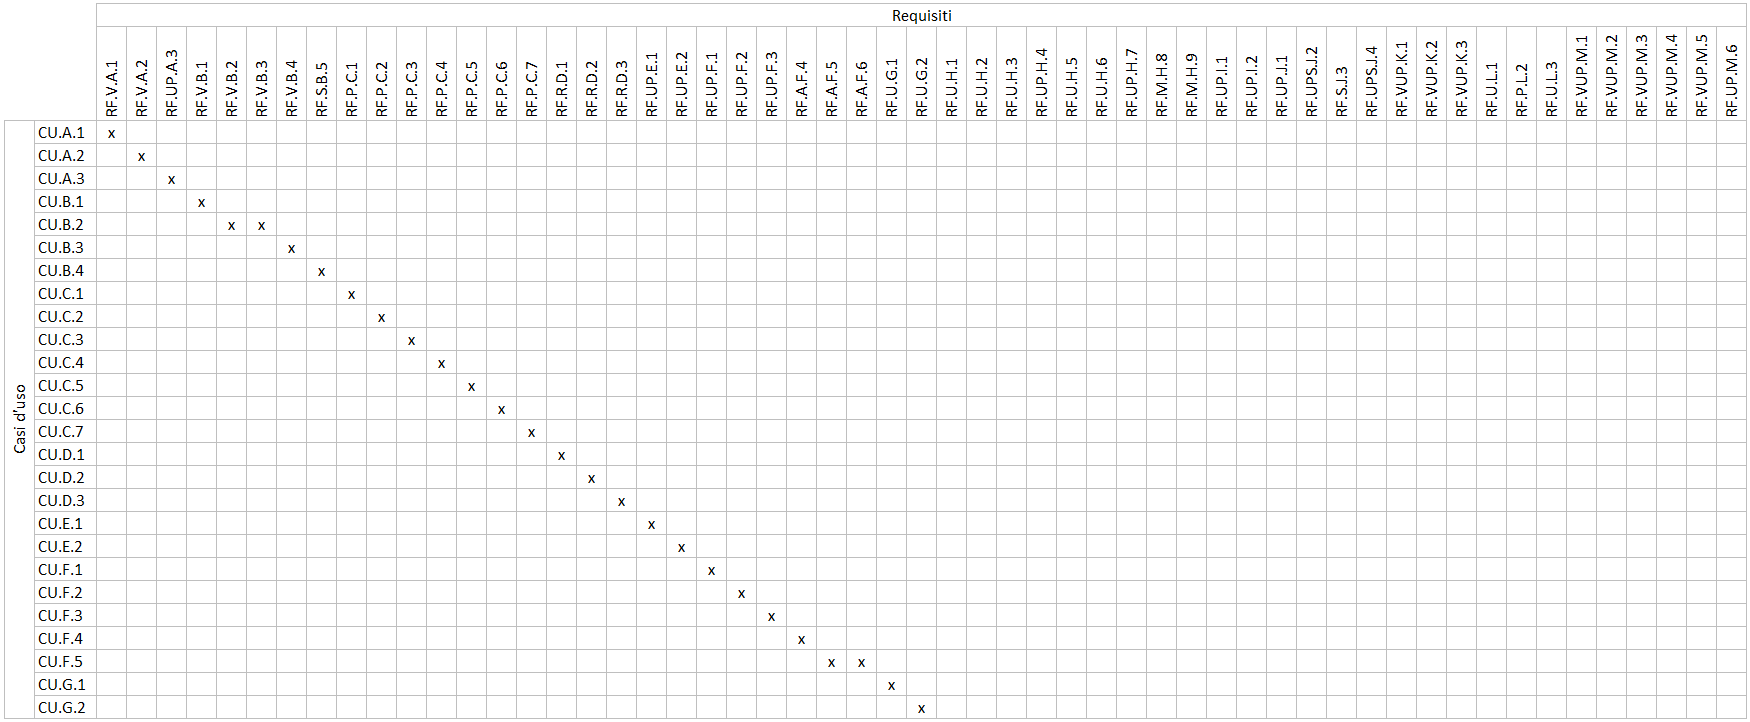
\includegraphics[width=\linewidth]{assets/matricetracciabilita0}
\end{center}
\end{landscape}

\begin{landscape}
\begin{center}
	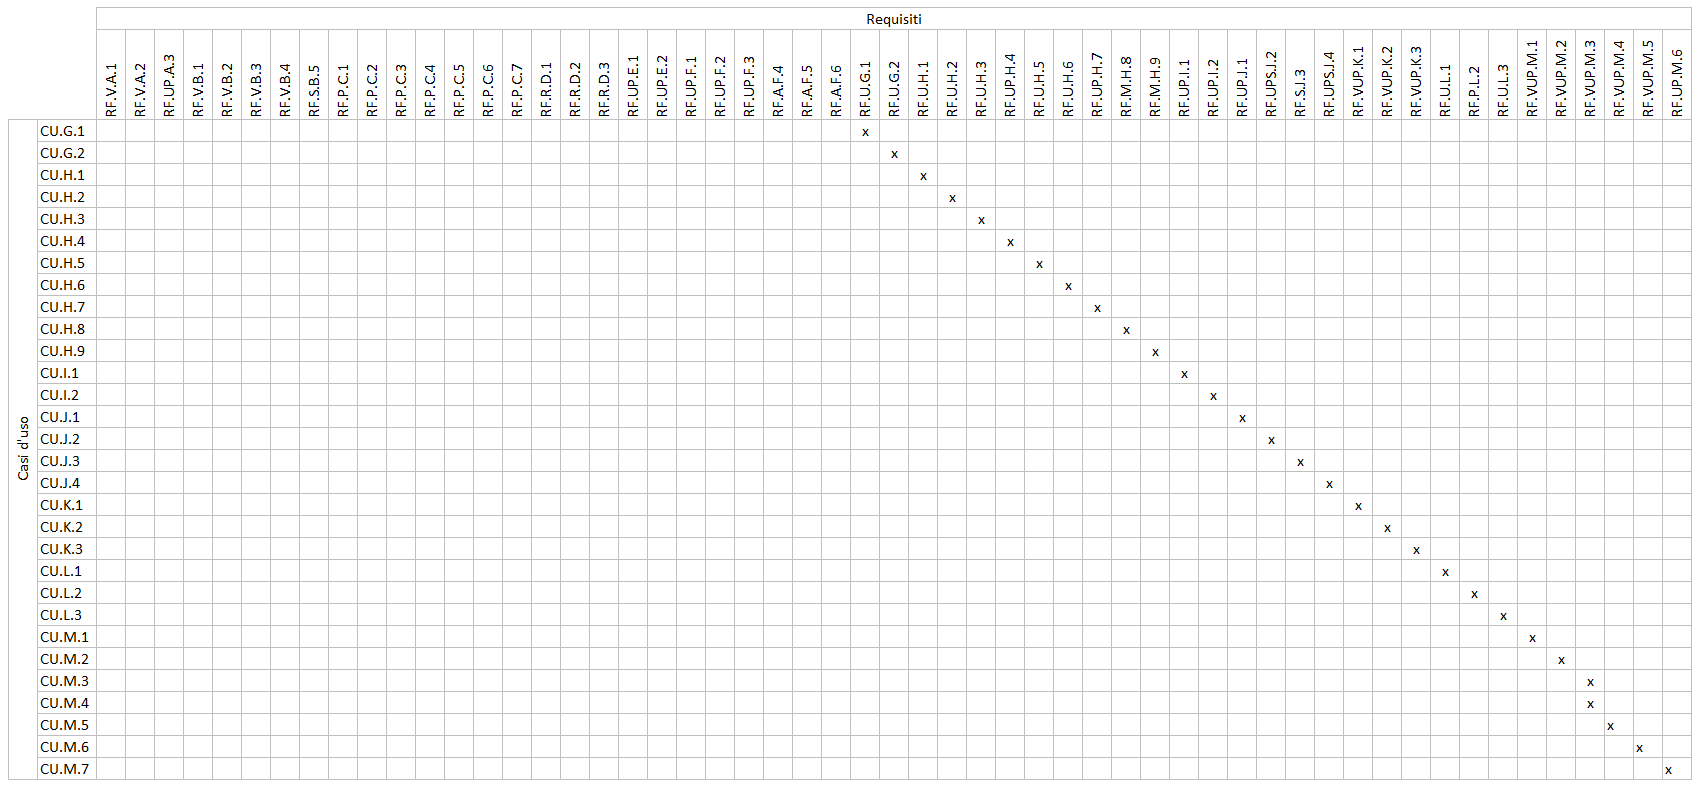
\includegraphics[width=\linewidth]{assets/matricetracciabilita1}
\end{center}
\end{landscape}

\newdate{cuuno}{12}{09}{2016}
\newdate{cudue}{29}{09}{2016}
\section{Revisioni}
\begin{center}
    \begin{tabular}{lll}
        \toprule
        	\tabhead{Versione} & \tabhead{Data} & \tabhead{Descrizione} \\
		\cmidrule(l{\cmidrulekern}r{\cmidrulekern}){1-3}
        	1.0 & \displaydate{cuuno} & Prima versione \\
        	1.1 & \displaydate{cudue} & Riorganizzati casi d'uso \\
        \bottomrule
    \end{tabular}
\end{center}